%%%%%%%% ICML 2025 EXAMPLE LATEX SUBMISSION FILE %%%%%%%%%%%%%%%%%

\documentclass{article}

% Recommended, but optional, packages for figures and better typesetting:
\usepackage{microtype}
\usepackage{graphicx}
\usepackage{subfigure}
\usepackage{booktabs} % for professional tables

% hyperref makes hyperlinks in the resulting PDF.
% If your build breaks (sometimes temporarily if a hyperlink spans a page)
% please comment out the following usepackage line and replace
% \usepackage{icml2025} with \usepackage[nohyperref]{icml2025} above.
\usepackage{hyperref}


% Attempt to make hyperref and algorithmic work together better:
\newcommand{\theHalgorithm}{\arabic{algorithm}}

% Use the following line for the initial blind version submitted for review:
%\usepackage{icml2025}

% If accepted, instead use the following line for the camera-ready submission:
\usepackage[accepted]{icml2025}

% For theorems and such
\usepackage{amsmath}
\usepackage{amssymb}
\usepackage{mathtools}
\usepackage{amsthm}

% if you use cleveref..
\usepackage[capitalize,noabbrev]{cleveref}

\usepackage{tabularx} % Add this in your preamble

%%%%%%%%%%%%%%%%%%%%%%%%%%%%%%%%
% THEOREMS
%%%%%%%%%%%%%%%%%%%%%%%%%%%%%%%%
\theoremstyle{plain}
\newtheorem{theorem}{Theorem}[section]
\newtheorem{proposition}[theorem]{Proposition}
\newtheorem{lemma}[theorem]{Lemma}
\newtheorem{corollary}[theorem]{Corollary}
\theoremstyle{definition}
\newtheorem{definition}[theorem]{Definition}
\newtheorem{assumption}[theorem]{Assumption}
\theoremstyle{remark}
\newtheorem{remark}[theorem]{Remark}

% Todonotes is useful during development; simply uncomment the next line
%    and comment out the line below the next line to turn off comments
%\usepackage[disable,textsize=tiny]{todonotes}
\usepackage[textsize=tiny]{todonotes}


%myPackages
\usepackage{multirow}
\usepackage{booktabs}
\usepackage{tabularx}

% The \icmltitle you define below is probably too long as a header.
% Therefore, a short form for the running title is supplied here:
\icmltitlerunning{iVISPAR — An Interactive Visual-Spatial Reasoning Benchmark for VLMs}

\begin{document}

\twocolumn[
\icmltitle{iVISPAR — An Interactive Visual-Spatial Reasoning Benchmark for VLMs}

% It is OKAY to include author information, even for blind
% submissions: the style file will automatically remove it for you
% unless you've provided the [accepted] option to the icml2025
% package.

% List of affiliations: The first argument should be a (short)
% identifier you will use later to specify author affiliations
% Academic affiliations should list Department, University, City, Region, Country
% Industry affiliations should list Company, City, Region, Country

% You can specify symbols, otherwise they are numbered in order.
% Ideally, you should not use this facility. Affiliations will be numbered
% in order of appearance and this is the preferred way.
\icmlsetsymbol{equal}{*}

\begin{icmlauthorlist}
\icmlauthor{Julius Mayer}{uos}
\icmlauthor{Mohamad Ballout}{uos,equal}
\icmlauthor{Serwan Jassim}{uos,equal}
\icmlauthor{Farbod Nosrat Nezami}{uos,equal}
\icmlauthor{Elia Bruni}{uos}
\newline %added by myself for anonymous version
\href{https://ivispar.ai}{https://ivispar.ai}
\end{icmlauthorlist}

\icmlaffiliation{uos}{Institute of Cognitive Science, University of Osnabrück, Osnabrück, Germany}


\icmlcorrespondingauthor{Julius Mayer}{research@jmayer.ai}

% You may provide any keywords that you
% find helpful for describing your paper; these are used to populate
% the "keywords" metadata in the PDF but will not be shown in the document
\icmlkeywords{benchmark, spatial-reasoning, visual-reasoning, vision-large-language-models}

\vskip 0.3in
]


\newcommand{\elia}[1]{%
  {\color{cyan!70!blue}[\textbf{Elia:} #1]}%
}

\newcommand{\Mohamad}[1]{%
  {\color{cyan!70!blue}[\textbf{Mohamad:} #1]}%
}

\newcommand{\Julius}[1]{%
  {\color{cyan!70!blue}[\textbf{Julius:} #1]}%
}

\newcommand{\Serwan}[1]{%
  {\color{cyan!70!blue}[\textbf{Serwan:} #1]}%
}

% this must go after the closing bracket ] following \twocolumn[ ...

% This command actually creates the footnote in the first column
% listing the affiliations and the copyright notice.
% The command takes one argument, which is text to display at the start of the footnote.
% The \icmlEqualContribution command is standard text for equal contribution.
% Remove it (just {}) if you do not need this facility.

%\printAffiliationsAndNotice{}  % leave blank if no need to mention equal contribution
\printAffiliationsAndNotice{\icmlEqualContribution} % otherwise use the standard text.

%my own
%\renewcommand{\thefootnote}{\fnsymbol{footnote}}
\footnotetext[1]{Correspondence to: J. Mayer $<$\texttt{research@jmayer.ai}$>$}
\renewcommand{\thefootnote}{\arabic{footnote}}

%%%%%%%%%%%%%%%%%%%%%%%%%%%%%%%%
% Abstract
%%%%%%%%%%%%%%%%%%%%%%%%%%%%%%%%

\begin{abstract}
AI systems are increasingly used to support human decision-making. In many cases, despite the algorithm's superior performance, the final decision remains in human hands. For example, an AI may assist doctors in determining which diagnostic tests to run, but the doctor ultimately makes the diagnosis. Focusing on these scenarios, this paper studies AI-assisted decision-making where the human learns through repeated interactions with the algorithm. In our framework, the algorithm -- designed to maximize decision accuracy according to its own model -- determines which features the human can consider. The human then makes a prediction based on their own less accurate model. Additionally, we consider the possibility of a constraint on the number of features that can be taken into account.


We observe that the discrepancy between the algorithm's model and the human's model creates a fundamental trade-off. Should the algorithm prioritize recommending more informative features, encouraging the human to recognize their importance, even if it results in less accurate predictions in the short term until learning occurs? Or is it preferable to forgo educating the human and instead select features that align more closely with their existing understanding, minimizing the immediate cost of learning? 
This trade-off is shaped by both the algorithm's patience (the time-discount rate of its objective function over multiple periods) and the human's willingness and ability to learn.


Our results show that optimal feature selection has a surprisingly clean combinatorial characterization, reducible to a stationary sequence of feature subsets that is tractable to compute.
As the algorithm becomes more patient or the human's learning improves, the algorithm increasingly selects more informative features, enhancing both prediction accuracy and the human's understanding of the world. Notably, early investment in learning leads to the selection of more informative features compared to a later investment. We complement our analysis by showing that the impact of errors in the algorithm's knowledge is limited as it does not make the prediction directly. 


\end{abstract}

%intro figure with overall results

%intro figure with overall results
\begin{figure}[h]
   \vskip 0.2in
    \begin{center}
        \centerline{
            \begin{minipage}{\linewidth}
                \centering
                \includegraphics[width=\linewidth]{imgs/graphs/stacked_bar_plot_won.png}
            \end{minipage}
        }
        \caption{VLMs' success rates of completed games over 900 episodes across all modalities: vision 3D, vision 2D, and text.}
        \label{fig:stacked_bar_plot_win_percentage}
    \end{center}
    \vskip -0.2in
\end{figure}


%%%%%%%%%%%%%%%%%%%%%%%%%%%%%%%%
% Introduction
%%%%%%%%%%%%%%%%%%%%%%%%%%%%%%%%
\section{Introduction}

\label{introduction}
\section{Introduction}
\label{sec:introduction}
The business processes of organizations are experiencing ever-increasing complexity due to the large amount of data, high number of users, and high-tech devices involved \cite{martin2021pmopportunitieschallenges, beerepoot2023biggestbpmproblems}. This complexity may cause business processes to deviate from normal control flow due to unforeseen and disruptive anomalies \cite{adams2023proceddsriftdetection}. These control-flow anomalies manifest as unknown, skipped, and wrongly-ordered activities in the traces of event logs monitored from the execution of business processes \cite{ko2023adsystematicreview}. For the sake of clarity, let us consider an illustrative example of such anomalies. Figure \ref{FP_ANOMALIES} shows a so-called event log footprint, which captures the control flow relations of four activities of a hypothetical event log. In particular, this footprint captures the control-flow relations between activities \texttt{a}, \texttt{b}, \texttt{c} and \texttt{d}. These are the causal ($\rightarrow$) relation, concurrent ($\parallel$) relation, and other ($\#$) relations such as exclusivity or non-local dependency \cite{aalst2022pmhandbook}. In addition, on the right are six traces, of which five exhibit skipped, wrongly-ordered and unknown control-flow anomalies. For example, $\langle$\texttt{a b d}$\rangle$ has a skipped activity, which is \texttt{c}. Because of this skipped activity, the control-flow relation \texttt{b}$\,\#\,$\texttt{d} is violated, since \texttt{d} directly follows \texttt{b} in the anomalous trace.
\begin{figure}[!t]
\centering
\includegraphics[width=0.9\columnwidth]{images/FP_ANOMALIES.png}
\caption{An example event log footprint with six traces, of which five exhibit control-flow anomalies.}
\label{FP_ANOMALIES}
\end{figure}

\subsection{Control-flow anomaly detection}
Control-flow anomaly detection techniques aim to characterize the normal control flow from event logs and verify whether these deviations occur in new event logs \cite{ko2023adsystematicreview}. To develop control-flow anomaly detection techniques, \revision{process mining} has seen widespread adoption owing to process discovery and \revision{conformance checking}. On the one hand, process discovery is a set of algorithms that encode control-flow relations as a set of model elements and constraints according to a given modeling formalism \cite{aalst2022pmhandbook}; hereafter, we refer to the Petri net, a widespread modeling formalism. On the other hand, \revision{conformance checking} is an explainable set of algorithms that allows linking any deviations with the reference Petri net and providing the fitness measure, namely a measure of how much the Petri net fits the new event log \cite{aalst2022pmhandbook}. Many control-flow anomaly detection techniques based on \revision{conformance checking} (hereafter, \revision{conformance checking}-based techniques) use the fitness measure to determine whether an event log is anomalous \cite{bezerra2009pmad, bezerra2013adlogspais, myers2018icsadpm, pecchia2020applicationfailuresanalysispm}. 

The scientific literature also includes many \revision{conformance checking}-independent techniques for control-flow anomaly detection that combine specific types of trace encodings with machine/deep learning \cite{ko2023adsystematicreview, tavares2023pmtraceencoding}. Whereas these techniques are very effective, their explainability is challenging due to both the type of trace encoding employed and the machine/deep learning model used \cite{rawal2022trustworthyaiadvances,li2023explainablead}. Hence, in the following, we focus on the shortcomings of \revision{conformance checking}-based techniques to investigate whether it is possible to support the development of competitive control-flow anomaly detection techniques while maintaining the explainable nature of \revision{conformance checking}.
\begin{figure}[!t]
\centering
\includegraphics[width=\columnwidth]{images/HIGH_LEVEL_VIEW.png}
\caption{A high-level view of the proposed framework for combining \revision{process mining}-based feature extraction with dimensionality reduction for control-flow anomaly detection.}
\label{HIGH_LEVEL_VIEW}
\end{figure}

\subsection{Shortcomings of \revision{conformance checking}-based techniques}
Unfortunately, the detection effectiveness of \revision{conformance checking}-based techniques is affected by noisy data and low-quality Petri nets, which may be due to human errors in the modeling process or representational bias of process discovery algorithms \cite{bezerra2013adlogspais, pecchia2020applicationfailuresanalysispm, aalst2016pm}. Specifically, on the one hand, noisy data may introduce infrequent and deceptive control-flow relations that may result in inconsistent fitness measures, whereas, on the other hand, checking event logs against a low-quality Petri net could lead to an unreliable distribution of fitness measures. Nonetheless, such Petri nets can still be used as references to obtain insightful information for \revision{process mining}-based feature extraction, supporting the development of competitive and explainable \revision{conformance checking}-based techniques for control-flow anomaly detection despite the problems above. For example, a few works outline that token-based \revision{conformance checking} can be used for \revision{process mining}-based feature extraction to build tabular data and develop effective \revision{conformance checking}-based techniques for control-flow anomaly detection \cite{singh2022lapmsh, debenedictis2023dtadiiot}. However, to the best of our knowledge, the scientific literature lacks a structured proposal for \revision{process mining}-based feature extraction using the state-of-the-art \revision{conformance checking} variant, namely alignment-based \revision{conformance checking}.

\subsection{Contributions}
We propose a novel \revision{process mining}-based feature extraction approach with alignment-based \revision{conformance checking}. This variant aligns the deviating control flow with a reference Petri net; the resulting alignment can be inspected to extract additional statistics such as the number of times a given activity caused mismatches \cite{aalst2022pmhandbook}. We integrate this approach into a flexible and explainable framework for developing techniques for control-flow anomaly detection. The framework combines \revision{process mining}-based feature extraction and dimensionality reduction to handle high-dimensional feature sets, achieve detection effectiveness, and support explainability. Notably, in addition to our proposed \revision{process mining}-based feature extraction approach, the framework allows employing other approaches, enabling a fair comparison of multiple \revision{conformance checking}-based and \revision{conformance checking}-independent techniques for control-flow anomaly detection. Figure \ref{HIGH_LEVEL_VIEW} shows a high-level view of the framework. Business processes are monitored, and event logs obtained from the database of information systems. Subsequently, \revision{process mining}-based feature extraction is applied to these event logs and tabular data input to dimensionality reduction to identify control-flow anomalies. We apply several \revision{conformance checking}-based and \revision{conformance checking}-independent framework techniques to publicly available datasets, simulated data of a case study from railways, and real-world data of a case study from healthcare. We show that the framework techniques implementing our approach outperform the baseline \revision{conformance checking}-based techniques while maintaining the explainable nature of \revision{conformance checking}.

In summary, the contributions of this paper are as follows.
\begin{itemize}
    \item{
        A novel \revision{process mining}-based feature extraction approach to support the development of competitive and explainable \revision{conformance checking}-based techniques for control-flow anomaly detection.
    }
    \item{
        A flexible and explainable framework for developing techniques for control-flow anomaly detection using \revision{process mining}-based feature extraction and dimensionality reduction.
    }
    \item{
        Application to synthetic and real-world datasets of several \revision{conformance checking}-based and \revision{conformance checking}-independent framework techniques, evaluating their detection effectiveness and explainability.
    }
\end{itemize}

The rest of the paper is organized as follows.
\begin{itemize}
    \item Section \ref{sec:related_work} reviews the existing techniques for control-flow anomaly detection, categorizing them into \revision{conformance checking}-based and \revision{conformance checking}-independent techniques.
    \item Section \ref{sec:abccfe} provides the preliminaries of \revision{process mining} to establish the notation used throughout the paper, and delves into the details of the proposed \revision{process mining}-based feature extraction approach with alignment-based \revision{conformance checking}.
    \item Section \ref{sec:framework} describes the framework for developing \revision{conformance checking}-based and \revision{conformance checking}-independent techniques for control-flow anomaly detection that combine \revision{process mining}-based feature extraction and dimensionality reduction.
    \item Section \ref{sec:evaluation} presents the experiments conducted with multiple framework and baseline techniques using data from publicly available datasets and case studies.
    \item Section \ref{sec:conclusions} draws the conclusions and presents future work.
\end{itemize}

%Figure
\begin{figure*}[ht]
    \vskip 0.2in
    \begin{center}
        \centerline{
            \begin{minipage}{0.33\linewidth}
                \centering
                \includegraphics[width=\linewidth]{imgs/game_vis/SGP_state_active_border.png}
            \end{minipage}
            \hfill
            \begin{minipage}{0.33\linewidth}
                \centering
                \includegraphics[width=\linewidth]{imgs/game_vis/2_current_border.png}
            \end{minipage}
            \hfill
            \begin{minipage}{0.33\linewidth}
                \centering
                \includegraphics[width=\linewidth]{imgs/game_vis/text_active.png}
            \end{minipage}
        }
        \vskip 0.1in
        \centerline{
            \begin{minipage}{0.33\linewidth}
                \centering
                \includegraphics[width=\linewidth]{imgs/game_vis/SGP_state_goal_border.png}
            \end{minipage}
            \hfill
            \begin{minipage}{0.33\linewidth}
                \centering
                \includegraphics[width=\linewidth]{imgs/game_vis/2_goal_border.png}
            \end{minipage}
            \hfill
            \begin{minipage}{0.33\linewidth}
                \centering
                \includegraphics[width=\linewidth]{imgs/game_vis/text_goal.png}
            \end{minipage}
        }
        \caption{Visualizations of VLMs' observations for the active and goal states for all modalities: vision 3D (left), vision 2D (middle), text-base representation, provided to models as a string (right) on a 4x4 board at each step during the Sliding Geom Puzzle environment.}
        \label{fig:SGP_states}
    \end{center}
    \vskip -0.2in
\end{figure*}


%%%%%%%%%%%%%%%%%%%%%%%%%%%%%%%%
% Related work
%%%%%%%%%%%%%%%%%%%%%%%%%%%%%%%%
\section{Related work}
\label{relatedwork}
\section{RELATED WORK}
\label{sec:relatedwork}
In this section, we describe the previous works related to our proposal, which are divided into two parts. In Section~\ref{sec:relatedwork_exoplanet}, we present a review of approaches based on machine learning techniques for the detection of planetary transit signals. Section~\ref{sec:relatedwork_attention} provides an account of the approaches based on attention mechanisms applied in Astronomy.\par

\subsection{Exoplanet detection}
\label{sec:relatedwork_exoplanet}
Machine learning methods have achieved great performance for the automatic selection of exoplanet transit signals. One of the earliest applications of machine learning is a model named Autovetter \citep{MCcauliff}, which is a random forest (RF) model based on characteristics derived from Kepler pipeline statistics to classify exoplanet and false positive signals. Then, other studies emerged that also used supervised learning. \cite{mislis2016sidra} also used a RF, but unlike the work by \citet{MCcauliff}, they used simulated light curves and a box least square \citep[BLS;][]{kovacs2002box}-based periodogram to search for transiting exoplanets. \citet{thompson2015machine} proposed a k-nearest neighbors model for Kepler data to determine if a given signal has similarity to known transits. Unsupervised learning techniques were also applied, such as self-organizing maps (SOM), proposed \citet{armstrong2016transit}; which implements an architecture to segment similar light curves. In the same way, \citet{armstrong2018automatic} developed a combination of supervised and unsupervised learning, including RF and SOM models. In general, these approaches require a previous phase of feature engineering for each light curve. \par

%DL is a modern data-driven technology that automatically extracts characteristics, and that has been successful in classification problems from a variety of application domains. The architecture relies on several layers of NNs of simple interconnected units and uses layers to build increasingly complex and useful features by means of linear and non-linear transformation. This family of models is capable of generating increasingly high-level representations \citep{lecun2015deep}.

The application of DL for exoplanetary signal detection has evolved rapidly in recent years and has become very popular in planetary science.  \citet{pearson2018} and \citet{zucker2018shallow} developed CNN-based algorithms that learn from synthetic data to search for exoplanets. Perhaps one of the most successful applications of the DL models in transit detection was that of \citet{Shallue_2018}; who, in collaboration with Google, proposed a CNN named AstroNet that recognizes exoplanet signals in real data from Kepler. AstroNet uses the training set of labelled TCEs from the Autovetter planet candidate catalog of Q1–Q17 data release 24 (DR24) of the Kepler mission \citep{catanzarite2015autovetter}. AstroNet analyses the data in two views: a ``global view'', and ``local view'' \citep{Shallue_2018}. \par


% The global view shows the characteristics of the light curve over an orbital period, and a local view shows the moment at occurring the transit in detail

%different = space-based

Based on AstroNet, researchers have modified the original AstroNet model to rank candidates from different surveys, specifically for Kepler and TESS missions. \citet{ansdell2018scientific} developed a CNN trained on Kepler data, and included for the first time the information on the centroids, showing that the model improves performance considerably. Then, \citet{osborn2020rapid} and \citet{yu2019identifying} also included the centroids information, but in addition, \citet{osborn2020rapid} included information of the stellar and transit parameters. Finally, \citet{rao2021nigraha} proposed a pipeline that includes a new ``half-phase'' view of the transit signal. This half-phase view represents a transit view with a different time and phase. The purpose of this view is to recover any possible secondary eclipse (the object hiding behind the disk of the primary star).


%last pipeline applies a procedure after the prediction of the model to obtain new candidates, this process is carried out through a series of steps that include the evaluation with Discovery and Validation of Exoplanets (DAVE) \citet{kostov2019discovery} that was adapted for the TESS telescope.\par
%



\subsection{Attention mechanisms in astronomy}
\label{sec:relatedwork_attention}
Despite the remarkable success of attention mechanisms in sequential data, few papers have exploited their advantages in astronomy. In particular, there are no models based on attention mechanisms for detecting planets. Below we present a summary of the main applications of this modeling approach to astronomy, based on two points of view; performance and interpretability of the model.\par
%Attention mechanisms have not yet been explored in all sub-areas of astronomy. However, recent works show a successful application of the mechanism.
%performance

The application of attention mechanisms has shown improvements in the performance of some regression and classification tasks compared to previous approaches. One of the first implementations of the attention mechanism was to find gravitational lenses proposed by \citet{thuruthipilly2021finding}. They designed 21 self-attention-based encoder models, where each model was trained separately with 18,000 simulated images, demonstrating that the model based on the Transformer has a better performance and uses fewer trainable parameters compared to CNN. A novel application was proposed by \citet{lin2021galaxy} for the morphological classification of galaxies, who used an architecture derived from the Transformer, named Vision Transformer (VIT) \citep{dosovitskiy2020image}. \citet{lin2021galaxy} demonstrated competitive results compared to CNNs. Another application with successful results was proposed by \citet{zerveas2021transformer}; which first proposed a transformer-based framework for learning unsupervised representations of multivariate time series. Their methodology takes advantage of unlabeled data to train an encoder and extract dense vector representations of time series. Subsequently, they evaluate the model for regression and classification tasks, demonstrating better performance than other state-of-the-art supervised methods, even with data sets with limited samples.

%interpretation
Regarding the interpretability of the model, a recent contribution that analyses the attention maps was presented by \citet{bowles20212}, which explored the use of group-equivariant self-attention for radio astronomy classification. Compared to other approaches, this model analysed the attention maps of the predictions and showed that the mechanism extracts the brightest spots and jets of the radio source more clearly. This indicates that attention maps for prediction interpretation could help experts see patterns that the human eye often misses. \par

In the field of variable stars, \citet{allam2021paying} employed the mechanism for classifying multivariate time series in variable stars. And additionally, \citet{allam2021paying} showed that the activation weights are accommodated according to the variation in brightness of the star, achieving a more interpretable model. And finally, related to the TESS telescope, \citet{morvan2022don} proposed a model that removes the noise from the light curves through the distribution of attention weights. \citet{morvan2022don} showed that the use of the attention mechanism is excellent for removing noise and outliers in time series datasets compared with other approaches. In addition, the use of attention maps allowed them to show the representations learned from the model. \par

Recent attention mechanism approaches in astronomy demonstrate comparable results with earlier approaches, such as CNNs. At the same time, they offer interpretability of their results, which allows a post-prediction analysis. \par



%%%%%%%%%%%%%%%%%%%%%%%%%%%%%%%%
% The iVISPAR Benchmark
%%%%%%%%%%%%%%%%%%%%%%%%%%%%%%%%

%Figure

\begin{figure*}[h]
   \vskip 0.2in
    \begin{center}
        \centerline{
            \begin{minipage}{0.95\linewidth}
                \centering
                \includegraphics[width=\linewidth]{imgs/game_flow.png}
            \end{minipage}
        }
        \caption{Depiction of the interaction flow between VLM agents and the iVISPAR Simulator with a progression through an episode with the shortest path solution of 4 steps being solved by prompted actions from a VLM agent.}
        \label{fig:workflow}
    \end{center}
    \vskip -0.2in
\end{figure*}

\section{The iVISPAR Benchmark}
\label{ivisparbenchmark}
\section{Introduction}
\label{sec:introduction}
The business processes of organizations are experiencing ever-increasing complexity due to the large amount of data, high number of users, and high-tech devices involved \cite{martin2021pmopportunitieschallenges, beerepoot2023biggestbpmproblems}. This complexity may cause business processes to deviate from normal control flow due to unforeseen and disruptive anomalies \cite{adams2023proceddsriftdetection}. These control-flow anomalies manifest as unknown, skipped, and wrongly-ordered activities in the traces of event logs monitored from the execution of business processes \cite{ko2023adsystematicreview}. For the sake of clarity, let us consider an illustrative example of such anomalies. Figure \ref{FP_ANOMALIES} shows a so-called event log footprint, which captures the control flow relations of four activities of a hypothetical event log. In particular, this footprint captures the control-flow relations between activities \texttt{a}, \texttt{b}, \texttt{c} and \texttt{d}. These are the causal ($\rightarrow$) relation, concurrent ($\parallel$) relation, and other ($\#$) relations such as exclusivity or non-local dependency \cite{aalst2022pmhandbook}. In addition, on the right are six traces, of which five exhibit skipped, wrongly-ordered and unknown control-flow anomalies. For example, $\langle$\texttt{a b d}$\rangle$ has a skipped activity, which is \texttt{c}. Because of this skipped activity, the control-flow relation \texttt{b}$\,\#\,$\texttt{d} is violated, since \texttt{d} directly follows \texttt{b} in the anomalous trace.
\begin{figure}[!t]
\centering
\includegraphics[width=0.9\columnwidth]{images/FP_ANOMALIES.png}
\caption{An example event log footprint with six traces, of which five exhibit control-flow anomalies.}
\label{FP_ANOMALIES}
\end{figure}

\subsection{Control-flow anomaly detection}
Control-flow anomaly detection techniques aim to characterize the normal control flow from event logs and verify whether these deviations occur in new event logs \cite{ko2023adsystematicreview}. To develop control-flow anomaly detection techniques, \revision{process mining} has seen widespread adoption owing to process discovery and \revision{conformance checking}. On the one hand, process discovery is a set of algorithms that encode control-flow relations as a set of model elements and constraints according to a given modeling formalism \cite{aalst2022pmhandbook}; hereafter, we refer to the Petri net, a widespread modeling formalism. On the other hand, \revision{conformance checking} is an explainable set of algorithms that allows linking any deviations with the reference Petri net and providing the fitness measure, namely a measure of how much the Petri net fits the new event log \cite{aalst2022pmhandbook}. Many control-flow anomaly detection techniques based on \revision{conformance checking} (hereafter, \revision{conformance checking}-based techniques) use the fitness measure to determine whether an event log is anomalous \cite{bezerra2009pmad, bezerra2013adlogspais, myers2018icsadpm, pecchia2020applicationfailuresanalysispm}. 

The scientific literature also includes many \revision{conformance checking}-independent techniques for control-flow anomaly detection that combine specific types of trace encodings with machine/deep learning \cite{ko2023adsystematicreview, tavares2023pmtraceencoding}. Whereas these techniques are very effective, their explainability is challenging due to both the type of trace encoding employed and the machine/deep learning model used \cite{rawal2022trustworthyaiadvances,li2023explainablead}. Hence, in the following, we focus on the shortcomings of \revision{conformance checking}-based techniques to investigate whether it is possible to support the development of competitive control-flow anomaly detection techniques while maintaining the explainable nature of \revision{conformance checking}.
\begin{figure}[!t]
\centering
\includegraphics[width=\columnwidth]{images/HIGH_LEVEL_VIEW.png}
\caption{A high-level view of the proposed framework for combining \revision{process mining}-based feature extraction with dimensionality reduction for control-flow anomaly detection.}
\label{HIGH_LEVEL_VIEW}
\end{figure}

\subsection{Shortcomings of \revision{conformance checking}-based techniques}
Unfortunately, the detection effectiveness of \revision{conformance checking}-based techniques is affected by noisy data and low-quality Petri nets, which may be due to human errors in the modeling process or representational bias of process discovery algorithms \cite{bezerra2013adlogspais, pecchia2020applicationfailuresanalysispm, aalst2016pm}. Specifically, on the one hand, noisy data may introduce infrequent and deceptive control-flow relations that may result in inconsistent fitness measures, whereas, on the other hand, checking event logs against a low-quality Petri net could lead to an unreliable distribution of fitness measures. Nonetheless, such Petri nets can still be used as references to obtain insightful information for \revision{process mining}-based feature extraction, supporting the development of competitive and explainable \revision{conformance checking}-based techniques for control-flow anomaly detection despite the problems above. For example, a few works outline that token-based \revision{conformance checking} can be used for \revision{process mining}-based feature extraction to build tabular data and develop effective \revision{conformance checking}-based techniques for control-flow anomaly detection \cite{singh2022lapmsh, debenedictis2023dtadiiot}. However, to the best of our knowledge, the scientific literature lacks a structured proposal for \revision{process mining}-based feature extraction using the state-of-the-art \revision{conformance checking} variant, namely alignment-based \revision{conformance checking}.

\subsection{Contributions}
We propose a novel \revision{process mining}-based feature extraction approach with alignment-based \revision{conformance checking}. This variant aligns the deviating control flow with a reference Petri net; the resulting alignment can be inspected to extract additional statistics such as the number of times a given activity caused mismatches \cite{aalst2022pmhandbook}. We integrate this approach into a flexible and explainable framework for developing techniques for control-flow anomaly detection. The framework combines \revision{process mining}-based feature extraction and dimensionality reduction to handle high-dimensional feature sets, achieve detection effectiveness, and support explainability. Notably, in addition to our proposed \revision{process mining}-based feature extraction approach, the framework allows employing other approaches, enabling a fair comparison of multiple \revision{conformance checking}-based and \revision{conformance checking}-independent techniques for control-flow anomaly detection. Figure \ref{HIGH_LEVEL_VIEW} shows a high-level view of the framework. Business processes are monitored, and event logs obtained from the database of information systems. Subsequently, \revision{process mining}-based feature extraction is applied to these event logs and tabular data input to dimensionality reduction to identify control-flow anomalies. We apply several \revision{conformance checking}-based and \revision{conformance checking}-independent framework techniques to publicly available datasets, simulated data of a case study from railways, and real-world data of a case study from healthcare. We show that the framework techniques implementing our approach outperform the baseline \revision{conformance checking}-based techniques while maintaining the explainable nature of \revision{conformance checking}.

In summary, the contributions of this paper are as follows.
\begin{itemize}
    \item{
        A novel \revision{process mining}-based feature extraction approach to support the development of competitive and explainable \revision{conformance checking}-based techniques for control-flow anomaly detection.
    }
    \item{
        A flexible and explainable framework for developing techniques for control-flow anomaly detection using \revision{process mining}-based feature extraction and dimensionality reduction.
    }
    \item{
        Application to synthetic and real-world datasets of several \revision{conformance checking}-based and \revision{conformance checking}-independent framework techniques, evaluating their detection effectiveness and explainability.
    }
\end{itemize}

The rest of the paper is organized as follows.
\begin{itemize}
    \item Section \ref{sec:related_work} reviews the existing techniques for control-flow anomaly detection, categorizing them into \revision{conformance checking}-based and \revision{conformance checking}-independent techniques.
    \item Section \ref{sec:abccfe} provides the preliminaries of \revision{process mining} to establish the notation used throughout the paper, and delves into the details of the proposed \revision{process mining}-based feature extraction approach with alignment-based \revision{conformance checking}.
    \item Section \ref{sec:framework} describes the framework for developing \revision{conformance checking}-based and \revision{conformance checking}-independent techniques for control-flow anomaly detection that combine \revision{process mining}-based feature extraction and dimensionality reduction.
    \item Section \ref{sec:evaluation} presents the experiments conducted with multiple framework and baseline techniques using data from publicly available datasets and case studies.
    \item Section \ref{sec:conclusions} draws the conclusions and presents future work.
\end{itemize}

%Figure TODO add back in final version
%\begin{figure}[h]
    \vskip 0.2in
    \begin{center}
        \centerline{
            \begin{minipage}{0.32\linewidth}
                \centering
                \includegraphics[width=\linewidth]{imgs/game_vis/STP_state.png}
            \end{minipage}
            \begin{minipage}{0.32\linewidth}
                \centering
                \includegraphics[width=\linewidth]{imgs/game_vis/STP_goal.png}
            \end{minipage}
            \begin{minipage}{0.32\linewidth}
                \centering
                \includegraphics[width=\linewidth]{imgs/game_vis/obs_1.png}
            \end{minipage}
        }
        \caption{Left and middle: Visualization of an active and a goal state in a classic 15-tile Sliding Tile Puzzle on a 4x4 board, playable by agents within the iVISPAR benchmark. Right: Visualization of the complete geom set used for the experiments}
        \label{fig:STP_and_geom_vis}
    \end{center}
    \vskip -0.2in
\end{figure}

\subsection{Sliding Tile Puzzle}
\label{slidingtilepuzzle}
The sequential generalized sliding-tile puzzle (SGSTP) is a generalization of the classic 15-Tile Sliding Tile Puzzle (Appendix \ref{sec:geoms}: Figure \ref{fig:STP_and_geom_vis}). In the SGSTP, a set of \( n < m_1 \times m_2 \) tiles, each uniquely labeled \( 1, \dots, n \), are placed on a rectangular grid of size \( m_1 \times m_2 \), denoted by \( G = (V, E) \). The grid has \( m_1 \times m_2 - n \) empty positions that allow tile movement.  

A configuration of tiles is represented as an injective mapping from the set \( \{1, \dots, n\} \) to positions \( V = \{(v_x, v_y) : 1 \leq v_x \leq m_2, 1 \leq v_y \leq m_1 \} \). Each tile must be repositioned from an arbitrary initial configuration \( S = \{s_1, \dots, s_n\} \) to a specified goal configuration \( G = \{g_1, \dots, g_n\} \), such as an ordered row-major layout.  

Let the movement path of tile \( i \), where \( 1 \leq i \leq n \), be expressed as \( p_i : \mathbb{N}_0 \to V \). The puzzle seeks a set of feasible paths \( P = \{p_1, \dots, p_n\} \) that satisfy the following conditions for all \( 1 \leq i, j \leq n \) with \( i \neq j \), and for all time steps \( t \geq 0 \):  

\textbf{Incremental Movement:} \( p_i(t+1) = p_i(t) \text{ or } (p_i(t+1), p_i(t)) \in E \).  
    Tiles move to adjacent, unoccupied positions or stay still.  \\
\textbf{Goal Achievement:} \( p_i(0) = s_i \text{ and } p_i(T) = g_i \text{ for some } T \geq 0 \). 
    Each tile must start at \( s_i \) and reach \( g_i \). \\ 
\textbf{Exclusive Occupancy:} \( p_i(t) \neq p_j(t) \text{ for all } i \neq j \). 
    Two tiles cannot occupy the same position at the same time.  

In this sequential version, tiles move one at a time. Therefore, the head-on collision and corner-following constraints found in the generalized sliding-tile puzzle are omitted, as simultaneous tile movements are not permitted.

\subsection{Sliding Geom Puzzle}
\label{slidinggeompuzzle}
The Sliding Geom Puzzle (SGP) replaces traditional numbered tiles with geometric objects (geoms) that are uniquely defined by color and shape attributes, increasing visual-spatial complexity and enhancing task scalability. This design shift requires models to interpret object features rather than follow simple numerical sequences, mirroring real-world spatial reasoning, where objects are distinguished by appearance, size, or structure. This approach aligns with physical tasks such as organizing items, assembling structures, or packing, promoting a more authentic evaluation of real-world spatial capabilities.


\textbf{Game dynamics}\hspace{.3cm} In each episode, agents receive observations of the start and goal states, accompanied by task instructions. Agents apply move actions to geoms by referencing their unique color and shape combination and specifying the direction of intended movement. Geoms can be moved in cardinal directions (\textit{LEFT, RIGHT, UP, DOWN}), with actions formatted as "move $<$color$>$ $<$shape$>$ $<$direction$>$”:

\begin{verbatim}
"move blue sphere right"
\end{verbatim}

Actions are validated and applied if legal, with agents receiving updated board states regardless of the action’s success after each move command. Effective
and ineffective actions both result in valid new board states
but, respectively, decrease or increase the path length to
the goal state. Invalid moves, such as occupied destination
and out-of-bounds actions, fail to alter the board state, as
do illegal commands, which violate the instructed action
format. This action-perception loop repeats until the goal state is achieved or a step limit is reached. Due to limited context windows, VLM agents receive task instructions at each time step. System prompt instructions and a sample agent-environment interaction is provided in Appendix \ref{interaction}.

%empty line

%empty line
\textbf{Observation spaces}\hspace{.3cm} Agents observe a combination of the current board state and the goal state. Additionally they can receive a sequence of past state-action pairs, determined by the length of their context window. iVISPAR supports multi-modal observations of the board state, which can be represented in either a 3D vision, 2D vision or text-based modality (Figure \ref{fig:SGP_states}).Images for 3D and 2D vision modalities may optionally include embedded, text-based chess-style coordinate labels as spatial cues on outer edge of the grid board as well as on free tiles. Images can also marked with an embedded text label and a colored background to differentiate between past (grey), active (blue) and goal state (green). Figure \ref{fig:SGP_states} shows 3D vision (left) and 2D vision (middle) for the active state (top) and the goal state (bottom). Text-based representation encodes past, active, and goal states directly in the prompt string supplied to the agent. A visualization of the text-based active (top) and goal states (bottom) is shown in Figure \ref{fig:SGP_states} (right). Images are not used in this modality.
%empty line

%empty line
\textbf{Complexity scalability}\hspace{.3cm} GSTP is a well-known NP-hard problem due to the need for multi-step planning across a constrained grid \cite{gozon2024computing}. SGP inherits this complexity but introduces greater flexibility in scaling difficulty without altering the game’s core mechanics. This flexibility provides more degrees of freedom, making the task more tractable for VLM agents. Key scaling factors include board size, number of objects, object variability, length of the shortest path solution, and the geom interference factor (see Figure \ref{fig:SGP_scalibility}). The shortest path solution for all episode configurations is calculated using the A* algorithm \cite{hart1968formal}, as detailed in Appendix \ref{sec:optimal_agent}. The interference factor denotes the extent to which objects obstruct one another’s optimal paths, increasing the global solution length beyond the cumulative Manhattan distances of individual paths. This interference can create configurations with short optimal paths but increased planning requirements, significantly raising the problem's difficulty. Available geometric shapes include [“cube,” “pyramid,” “sphere,” “cylinder,” “cone,” “prism”], with colors freely selectable by referencing RGB values. Agents must navigate combinatorial complexity by matching shapes and colors, promoting spatial strategies over the sequential patterns seen in numerical tile puzzles. Episode configurations are randomly generated, requiring models to generalize across tasks. Human and algorithmic benchmarks for these experiments are detailed in Section \ref{sec:baselines}.


\textbf{Episode Configuration}\hspace{.3cm}  Unique episode configurations are generated by randomly sampling and pairing initial and goal states. These configurations are classified according to hyperparameters, including board size, number of geoms, shortest path solution length, and the geom interference factor (Appendix \ref{sec:params_configs}). Geoms on the board are assigned shape and color properties derived from the specified hyperparameter set. This structured approach facilitates the selection of episode datasets that accurately reflect targeted complexity requirements.


%%%%%%%%%%%%%%%%%%%%%%%%%%%%%%%%
% Experiments
%%%%%%%%%%%%%%%%%%%%%%%%%%%%%%%%
\section{Experiments}

%Figure
\begin{figure*}[ht]
    \vskip 0.2in
    \begin{center}
        \includegraphics[width=\linewidth]{imgs/graphs/barplot_won_with_baselines_and_ci.png}
        \vskip 0.2in
        \includegraphics[width=\linewidth]{imgs/graphs//barplot_spl_value_with_baselines_and_ci.png}
        \caption{VLM evaluation on 900 episodes per model across all three modalities, with 95\% confidence intervals. Baseline comparisons for human performance and random moves are shown. Top: VLMs' success rates of episodes completed with higher values denoting better performance. Bottom: VLMs' mean step deviation from the optimal path with lower values denoting better performance.}
        \label{fig:results_bar_plot}
    \end{center}
    \vskip -0.2in
\end{figure*}

\section{Introduction}
\label{sec:introduction}
The business processes of organizations are experiencing ever-increasing complexity due to the large amount of data, high number of users, and high-tech devices involved \cite{martin2021pmopportunitieschallenges, beerepoot2023biggestbpmproblems}. This complexity may cause business processes to deviate from normal control flow due to unforeseen and disruptive anomalies \cite{adams2023proceddsriftdetection}. These control-flow anomalies manifest as unknown, skipped, and wrongly-ordered activities in the traces of event logs monitored from the execution of business processes \cite{ko2023adsystematicreview}. For the sake of clarity, let us consider an illustrative example of such anomalies. Figure \ref{FP_ANOMALIES} shows a so-called event log footprint, which captures the control flow relations of four activities of a hypothetical event log. In particular, this footprint captures the control-flow relations between activities \texttt{a}, \texttt{b}, \texttt{c} and \texttt{d}. These are the causal ($\rightarrow$) relation, concurrent ($\parallel$) relation, and other ($\#$) relations such as exclusivity or non-local dependency \cite{aalst2022pmhandbook}. In addition, on the right are six traces, of which five exhibit skipped, wrongly-ordered and unknown control-flow anomalies. For example, $\langle$\texttt{a b d}$\rangle$ has a skipped activity, which is \texttt{c}. Because of this skipped activity, the control-flow relation \texttt{b}$\,\#\,$\texttt{d} is violated, since \texttt{d} directly follows \texttt{b} in the anomalous trace.
\begin{figure}[!t]
\centering
\includegraphics[width=0.9\columnwidth]{images/FP_ANOMALIES.png}
\caption{An example event log footprint with six traces, of which five exhibit control-flow anomalies.}
\label{FP_ANOMALIES}
\end{figure}

\subsection{Control-flow anomaly detection}
Control-flow anomaly detection techniques aim to characterize the normal control flow from event logs and verify whether these deviations occur in new event logs \cite{ko2023adsystematicreview}. To develop control-flow anomaly detection techniques, \revision{process mining} has seen widespread adoption owing to process discovery and \revision{conformance checking}. On the one hand, process discovery is a set of algorithms that encode control-flow relations as a set of model elements and constraints according to a given modeling formalism \cite{aalst2022pmhandbook}; hereafter, we refer to the Petri net, a widespread modeling formalism. On the other hand, \revision{conformance checking} is an explainable set of algorithms that allows linking any deviations with the reference Petri net and providing the fitness measure, namely a measure of how much the Petri net fits the new event log \cite{aalst2022pmhandbook}. Many control-flow anomaly detection techniques based on \revision{conformance checking} (hereafter, \revision{conformance checking}-based techniques) use the fitness measure to determine whether an event log is anomalous \cite{bezerra2009pmad, bezerra2013adlogspais, myers2018icsadpm, pecchia2020applicationfailuresanalysispm}. 

The scientific literature also includes many \revision{conformance checking}-independent techniques for control-flow anomaly detection that combine specific types of trace encodings with machine/deep learning \cite{ko2023adsystematicreview, tavares2023pmtraceencoding}. Whereas these techniques are very effective, their explainability is challenging due to both the type of trace encoding employed and the machine/deep learning model used \cite{rawal2022trustworthyaiadvances,li2023explainablead}. Hence, in the following, we focus on the shortcomings of \revision{conformance checking}-based techniques to investigate whether it is possible to support the development of competitive control-flow anomaly detection techniques while maintaining the explainable nature of \revision{conformance checking}.
\begin{figure}[!t]
\centering
\includegraphics[width=\columnwidth]{images/HIGH_LEVEL_VIEW.png}
\caption{A high-level view of the proposed framework for combining \revision{process mining}-based feature extraction with dimensionality reduction for control-flow anomaly detection.}
\label{HIGH_LEVEL_VIEW}
\end{figure}

\subsection{Shortcomings of \revision{conformance checking}-based techniques}
Unfortunately, the detection effectiveness of \revision{conformance checking}-based techniques is affected by noisy data and low-quality Petri nets, which may be due to human errors in the modeling process or representational bias of process discovery algorithms \cite{bezerra2013adlogspais, pecchia2020applicationfailuresanalysispm, aalst2016pm}. Specifically, on the one hand, noisy data may introduce infrequent and deceptive control-flow relations that may result in inconsistent fitness measures, whereas, on the other hand, checking event logs against a low-quality Petri net could lead to an unreliable distribution of fitness measures. Nonetheless, such Petri nets can still be used as references to obtain insightful information for \revision{process mining}-based feature extraction, supporting the development of competitive and explainable \revision{conformance checking}-based techniques for control-flow anomaly detection despite the problems above. For example, a few works outline that token-based \revision{conformance checking} can be used for \revision{process mining}-based feature extraction to build tabular data and develop effective \revision{conformance checking}-based techniques for control-flow anomaly detection \cite{singh2022lapmsh, debenedictis2023dtadiiot}. However, to the best of our knowledge, the scientific literature lacks a structured proposal for \revision{process mining}-based feature extraction using the state-of-the-art \revision{conformance checking} variant, namely alignment-based \revision{conformance checking}.

\subsection{Contributions}
We propose a novel \revision{process mining}-based feature extraction approach with alignment-based \revision{conformance checking}. This variant aligns the deviating control flow with a reference Petri net; the resulting alignment can be inspected to extract additional statistics such as the number of times a given activity caused mismatches \cite{aalst2022pmhandbook}. We integrate this approach into a flexible and explainable framework for developing techniques for control-flow anomaly detection. The framework combines \revision{process mining}-based feature extraction and dimensionality reduction to handle high-dimensional feature sets, achieve detection effectiveness, and support explainability. Notably, in addition to our proposed \revision{process mining}-based feature extraction approach, the framework allows employing other approaches, enabling a fair comparison of multiple \revision{conformance checking}-based and \revision{conformance checking}-independent techniques for control-flow anomaly detection. Figure \ref{HIGH_LEVEL_VIEW} shows a high-level view of the framework. Business processes are monitored, and event logs obtained from the database of information systems. Subsequently, \revision{process mining}-based feature extraction is applied to these event logs and tabular data input to dimensionality reduction to identify control-flow anomalies. We apply several \revision{conformance checking}-based and \revision{conformance checking}-independent framework techniques to publicly available datasets, simulated data of a case study from railways, and real-world data of a case study from healthcare. We show that the framework techniques implementing our approach outperform the baseline \revision{conformance checking}-based techniques while maintaining the explainable nature of \revision{conformance checking}.

In summary, the contributions of this paper are as follows.
\begin{itemize}
    \item{
        A novel \revision{process mining}-based feature extraction approach to support the development of competitive and explainable \revision{conformance checking}-based techniques for control-flow anomaly detection.
    }
    \item{
        A flexible and explainable framework for developing techniques for control-flow anomaly detection using \revision{process mining}-based feature extraction and dimensionality reduction.
    }
    \item{
        Application to synthetic and real-world datasets of several \revision{conformance checking}-based and \revision{conformance checking}-independent framework techniques, evaluating their detection effectiveness and explainability.
    }
\end{itemize}

The rest of the paper is organized as follows.
\begin{itemize}
    \item Section \ref{sec:related_work} reviews the existing techniques for control-flow anomaly detection, categorizing them into \revision{conformance checking}-based and \revision{conformance checking}-independent techniques.
    \item Section \ref{sec:abccfe} provides the preliminaries of \revision{process mining} to establish the notation used throughout the paper, and delves into the details of the proposed \revision{process mining}-based feature extraction approach with alignment-based \revision{conformance checking}.
    \item Section \ref{sec:framework} describes the framework for developing \revision{conformance checking}-based and \revision{conformance checking}-independent techniques for control-flow anomaly detection that combine \revision{process mining}-based feature extraction and dimensionality reduction.
    \item Section \ref{sec:evaluation} presents the experiments conducted with multiple framework and baseline techniques using data from publicly available datasets and case studies.
    \item Section \ref{sec:conclusions} draws the conclusions and presents future work.
\end{itemize}

\subsection{Dataset Generation}
\begin{algorithm}
\caption{A* Search Algorithm}
\label{alg:astar}
\begin{algorithmic}
    \REQUIRE Graph $G$, start node $s$, goal node $g$, heuristic function $h$
    \ENSURE Path from $s$ to $g$ (or failure)
    
    \STATE OpenSet $\gets \{s\}$
    \STATE ClosedSet $\gets \emptyset$
    \STATE $gScore[s] \gets 0$
    \STATE $fScore[s] \gets h(s)$
    \STATE CameFrom $\gets$ empty map
    
    \WHILE{OpenSet not empty}
        \STATE current $\gets$ node in OpenSet with lowest $fScore$
        \IF{current = g}
            \RETURN ReconstructPath(CameFrom, $g$)
        \ENDIF
        
        \STATE Remove current from OpenSet
        \STATE Add current to ClosedSet
        
        \FOR{each neighbor $n$ of current}
            \IF{$n \in$ ClosedSet}
                \STATE \textbf{continue}
            \ENDIF
            
            \STATE tentative\_gScore $\gets gScore[current] + \text{cost}(current, n)$
            
            \IF{$n \notin$ OpenSet}
                \STATE Add $n$ to OpenSet
            \ELSIF{tentative\_gScore $\geq gScore[n]$}
                \STATE \textbf{continue}
            \ENDIF
            
            \STATE CameFrom[$n$] $\gets$ current
            \STATE $gScore[n] \gets$ tentative\_gScore
            \STATE $fScore[n] \gets gScore[n] + h(n)$
        \ENDFOR
    \ENDWHILE

    \RETURN failure

\end{algorithmic}
\end{algorithm}

\subsection{Baselines}
\label{sec:baselines}
\begin{table}[h!]
    % \small
    \centering
    \caption{Links to baseline model checkpoints.}
    \resizebox{0.7\linewidth}{!}{
    \begin{tabular}{l|l}
    \toprule
    Model & URL \\
    \midrule
    Galactica 125M & \url{https://huggingface.co/facebook/galactica-125m}\\
    Galactica 1.3B& \url{https://huggingface.co/facebook/galactica-1.3b}\\
    Galactica 6.7B& \url{https://huggingface.co/facebook/galactica-6.7b}\\
    GIMLET & \url{https://huggingface.co/haitengzhao/gimlet}\\
    LlasMol & \url{https://huggingface.co/osunlp/LlaSMol-Mistral-7B}\\
    MolecularGPT & \url{https://huggingface.co/YuyanLiu/MolecularGPT}\\
    \bottomrule
    \end{tabular}}
    \label{app tab: baselines}
\end{table}

%Figure
\begin{figure*}[ht]
    \vskip 0.2in
    \begin{center}
        \includegraphics[width=\linewidth]{imgs/graphs/average_barplot_action_counts_with_ci.png}
        \vskip 0.2in
        \includegraphics[width=\linewidth]{imgs/graphs/average_barplot_action_counts_per_agent_with_ci.png}
        \caption{VLMs’ average action counts per episode. Effective / ineffective actions respectively decrease / increase the path length to the goal state. Occupied destination and out-of-bounds are invalid moves, while illegal commands break the instructed action format, all of which leave the board state unchanged. Top: Overall action counts for each modality. Bottom: Overall action counts for each model.}
        \label{fig:move_validity_double}
    \end{center}
    \vskip -0.2in
\end{figure*} 

\subsection{Models}
\label{sec:models}
% \vspace{-0.3cm}
\setlength{\tabcolsep}{0pt}
\renewcommand{\arraystretch}{0.95}
\setcounter{table}{1}
\begin{table*}[b]
    \small
    % \vspace{-5mm}
    \caption{Parametric models included in the experiments. Cond. = conditioning method, R.F. = receptive field in samples.
    PEQ = Parametric EQ, G = Gain, O = Offset, MLP = Multilayer Perceptron, RNL = Rational Non Linearity. Controllers: 
    .s = static, .d = dynamic, .sc = static conditional, .dc = dynamic conditional}
    \label{tab:models}
    % \vspace{-2mm}
    \centerline{
        \begin{tabular}{L{2.8cm}C{1.3cm}R{1.1cm}C{1.1cm}C{1.1cm}C{1.3cm}C{1.5cm}R{1.4cm}R{1.3cm}R{1.3cm}}
            \hline
            \hline
            Model
                & Cond.
                    & R.F.
                        & Blocks
                            & Kernel
                                & Dilation
                                    & Channels
                                        & \# Params 
                                            & FLOP/s 
                                                & MAC/s\\ 
            \hline
            TCN-F-45-S-16 & FiLM & 2047 & 5 & 7 & 4 & 16 & 15.0k & 736.5M & 364.3M\\
            TCN-TF-45-S-16 & TFiLM & 2047 & 5 & 7 & 4 & 16 & 42.0k & 762.8M & 364.2M\\
            TCN-TTF-45-S-16 & TTFiLM & 2047 & 5 & 7 & 4 & 16 & 17.3k & 744.0M & 367.4M\\
            TCN-TVF-45-S-16 & TVFiLM & 2047 & 5 & 7 & 4 & 16 & 17.7k & 740.4M & 366.2M\\
            \hline
            \hline
        \end{tabular}
    }
    \centerline{
        \begin{tabular}{L{2.8cm}C{1.3cm}R{1.1cm}C{1.2cm}C{2.3cm}C{1.5cm}R{1.4cm}R{1.3cm}R{1.3cm}}
            Model
                & Cond.
                    & R.F.
                        & Blocks
                            & State Dimension
                                & Channels
                                    & \# Params
                                        & FLOP/s 
                                            & MAC/s\\ 
            \hline
            S4-F-S-16 & FiLM & - & 4 & 4 & 16 & 8.9k & 135.2M & 53.8M\\
            S4-TF-S-16 & TFiLM & - & 4 & 4 & 16 & 30.0k & 155.6M & 53.8M\\
            S4-TTF-S-16 & TTFiLM & - & 4 & 4 & 16 & 10.2k & 141.0M & 56.3M\\
            S4-TVF-S-16 & TVFiLM & - & 4 & 4 & 16 & 11.6k & 138.9M & 55.3M\\
            \hline
            \hline
        \end{tabular}
    }
    \centerline{
        \begin{tabular}{L{3cm}C{7.2cm}R{1.4cm}R{1.3cm}R{1.3cm}}
            Model
                & Signal Chain
                    & \# Params
                        & FLOP/s 
                            & MAC/s\\
            \hline
            GB-C-DIST-MLP & PEQ.sc $\rightarrow$ G.sc $\rightarrow$ O.sc $\rightarrow$ MLP $\rightarrow$ G.sc $\rightarrow$ PEQ.sc & 4.5k & 202.8M & 101.4M\\
            GB-C-DIST-RNL & PEQ.sc $\rightarrow$ G.sc $\rightarrow$ O.sc $\rightarrow$ RNL $\rightarrow$ G.sc $\rightarrow$ PEQ.sc & 2.3k & 920.5k & 4.3k\\
            \hline
            GB-C-FUZZ-MLP & PEQ.sc $\rightarrow$ G.sc $\rightarrow$ O.dc $\rightarrow$ MLP $\rightarrow$ G.sc $\rightarrow$ PEQ.sc & 4.2k & 202.8M & 101.4M\\
            GB-C-FUZZ-RNL & PEQ.sc $\rightarrow$ G.sc $\rightarrow$ O.dc $\rightarrow$ RNL $\rightarrow$ G.sc $\rightarrow$ PEQ.sc & 2.0k & 988.9k & 3.6k\\
            \hline
            \hline
        \end{tabular}
    }
    % \vspace{-4mm}
\end{table*}

\subsection{Context-Aware Zero-Shot Reasoning}
The models employ Chain-of-Thought (CoT) reasoning \cite{wei2022chain} to break down complex problems into smaller sub-tasks, enhancing accuracy and interpretability (Appendix \ref{interaction}). We constrain VLMs’ context windows to the past two steps, incorporating state representations alongside the model’s action responses. This approach prioritizes extracting maximum value from limited experience to preserve the models’ sequential coherence and minimize computational overhead (Appendix \ref{sec:experiment_configs}). Operating within this context-aware zero-shot reasoning framework, the models interpret task requirements without examples,  drawing exclusively from pretrained knowledge, task instructions, and limited past interactions. 

\subsection{Evaluation}
\definecolor{darkgreen}{rgb}{0.0, 0.5, 0.0}
\definecolor{violet}{rgb}{0.56, 0.0, 1.0}
\section{Evaluation}
We apply our methodology to derive counterfactual policies for various MDPs, addressing three main research questions: (1) how does our policy's performance compare to the Gumbel-max SCM approach; (2) how do the counterfactual stability and monotonicity assumptions impact the probability bounds; and (3) how fast is our approach compared with the Gumbel-max SCM method?

\begin{figure*}
    \centering
    %
    \resizebox{0.6\textwidth}{!}{
        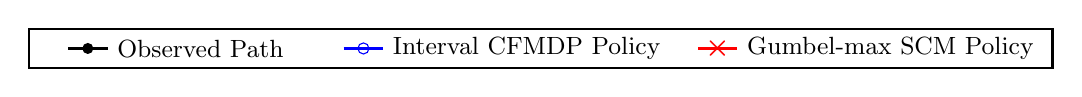
\begin{tikzpicture}[scale=1.0, every node/.style={scale=1.0}]
            \draw[thick, black] (-3, -0.25) rectangle (10, 0.25);
            %
            \draw[black, line width=1pt] (-2.5, 0.0) -- (-2,0.0);
            \fill[black] (-2.25,0.0) circle (2pt); %
            \node[right] at (-2,0.0) {\small Observed Path};
            
            %
            \draw[blue, line width=1pt] (1.0,0.0) -- (1.5,0.0);
            \node[draw=blue, circle, minimum size=4pt, inner sep=0pt] at (1.25,0.0) {}; %
            \node[right] at (1.5,0.0) {\small Interval CFMDP Policy};
            
            %
            \draw[red, line width=1pt] (5.5,0) -- (6,0);
            \node[red] at (5.75,0) {$\boldsymbol{\times}$}; %
            \node[right] at (6,0) {\small Gumbel-max SCM Policy};
        \end{tikzpicture}
    }\\
    %
    \subfigure[\footnotesize Lowest cumulative reward: Interval CFMDP ($312$), Gumbel-max SCM ($312$)]{%
        \resizebox{0.76\columnwidth}{!}{
             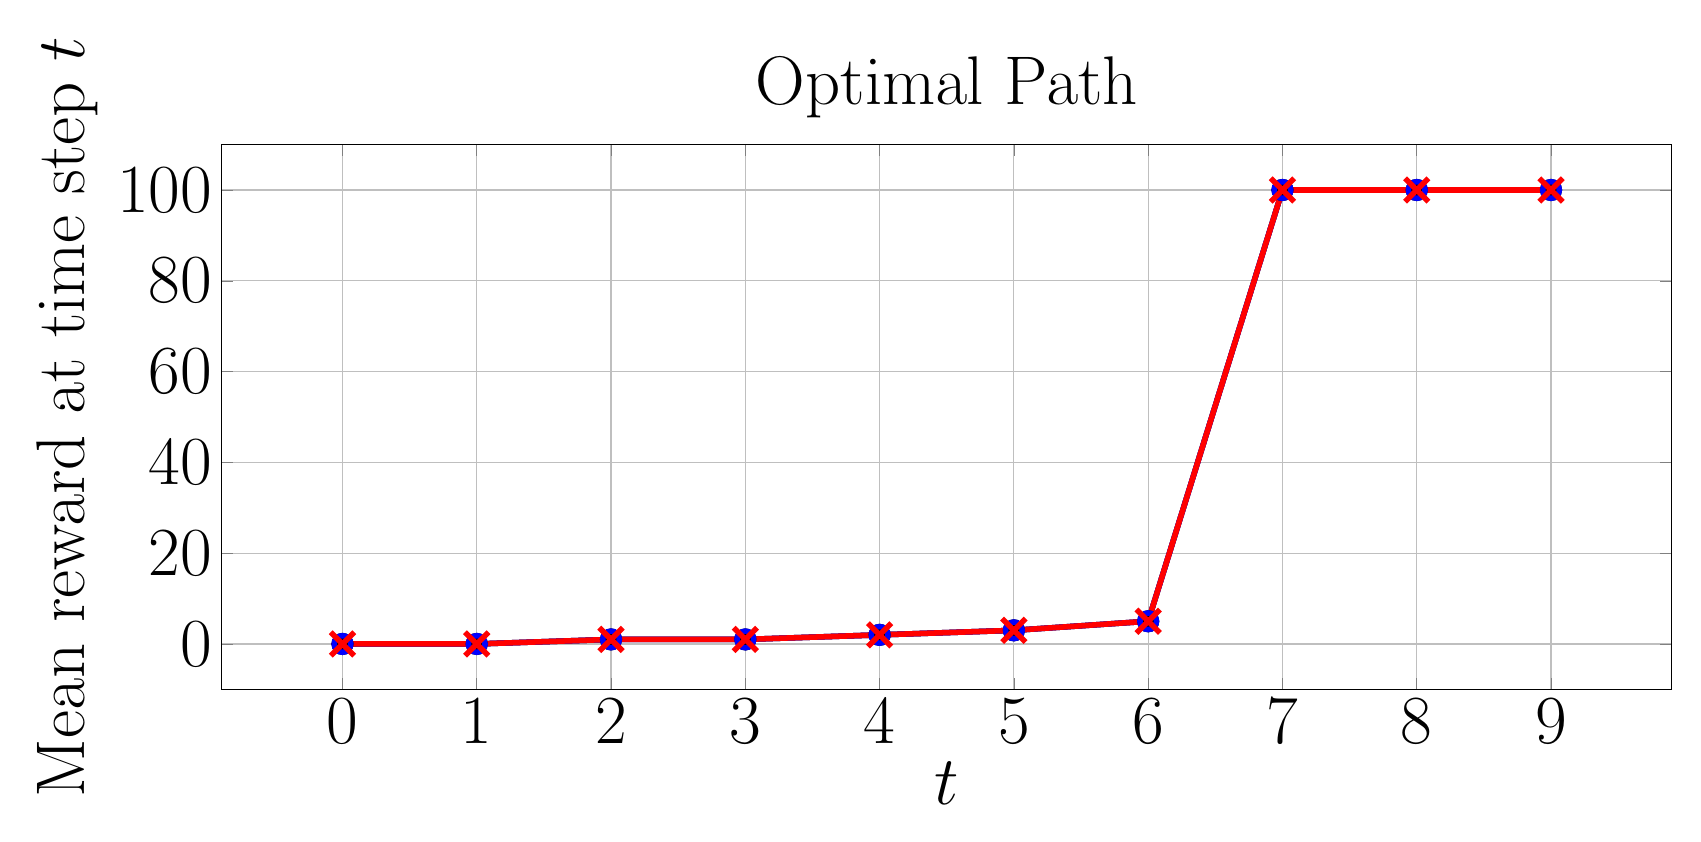
\begin{tikzpicture}
                \begin{axis}[
                    xlabel={$t$},
                    ylabel={Mean reward at time step $t$},
                    title={Optimal Path},
                    grid=both,
                    width=20cm, height=8.5cm,
                    every axis/.style={font=\Huge},
                    %
                ]
                \addplot[
                    color=black, %
                    mark=*, %
                    line width=2pt,
                    mark size=3pt,
                    error bars/.cd,
                    y dir=both, %
                    y explicit, %
                    error bar style={line width=1pt,solid},
                    error mark options={line width=1pt,mark size=4pt,rotate=90}
                ]
                coordinates {
                    (0, 0.0)  +- (0, 0.0)
                    (1, 0.0)  +- (0, 0.0) 
                    (2, 1.0)  +- (0, 0.0) 
                    (3, 1.0)  +- (0, 0.0)
                    (4, 2.0)  +- (0, 0.0)
                    (5, 3.0) +- (0, 0.0)
                    (6, 5.0) +- (0, 0.0)
                    (7, 100.0) +- (0, 0.0)
                    (8, 100.0) +- (0, 0.0)
                    (9, 100.0) +- (0, 0.0)
                };
                %
                \addplot[
                    color=blue, %
                    mark=o, %
                    line width=2pt,
                    mark size=3pt,
                    error bars/.cd,
                    y dir=both, %
                    y explicit, %
                    error bar style={line width=1pt,solid},
                    error mark options={line width=1pt,mark size=4pt,rotate=90}
                ]
                 coordinates {
                    (0, 0.0)  +- (0, 0.0)
                    (1, 0.0)  +- (0, 0.0) 
                    (2, 1.0)  +- (0, 0.0) 
                    (3, 1.0)  +- (0, 0.0)
                    (4, 2.0)  +- (0, 0.0)
                    (5, 3.0) +- (0, 0.0)
                    (6, 5.0) +- (0, 0.0)
                    (7, 100.0) +- (0, 0.0)
                    (8, 100.0) +- (0, 0.0)
                    (9, 100.0) +- (0, 0.0)
                };
                %
                \addplot[
                    color=red, %
                    mark=x, %
                    line width=2pt,
                    mark size=6pt,
                    error bars/.cd,
                    y dir=both, %
                    y explicit, %
                    error bar style={line width=1pt,solid},
                    error mark options={line width=1pt,mark size=4pt,rotate=90}
                ]
                coordinates {
                    (0, 0.0)  +- (0, 0.0)
                    (1, 0.0)  +- (0, 0.0) 
                    (2, 1.0)  +- (0, 0.0) 
                    (3, 1.0)  +- (0, 0.0)
                    (4, 2.0)  +- (0, 0.0)
                    (5, 3.0) +- (0, 0.0)
                    (6, 5.0) +- (0, 0.0)
                    (7, 100.0) +- (0, 0.0)
                    (8, 100.0) +- (0, 0.0)
                    (9, 100.0) +- (0, 0.0)
                };
                \end{axis}
            \end{tikzpicture}
         }
    }
    \hspace{1cm}
    \subfigure[\footnotesize Lowest cumulative reward: Interval CFMDP ($19$), Gumbel-max SCM ($-88$)]{%
         \resizebox{0.76\columnwidth}{!}{
            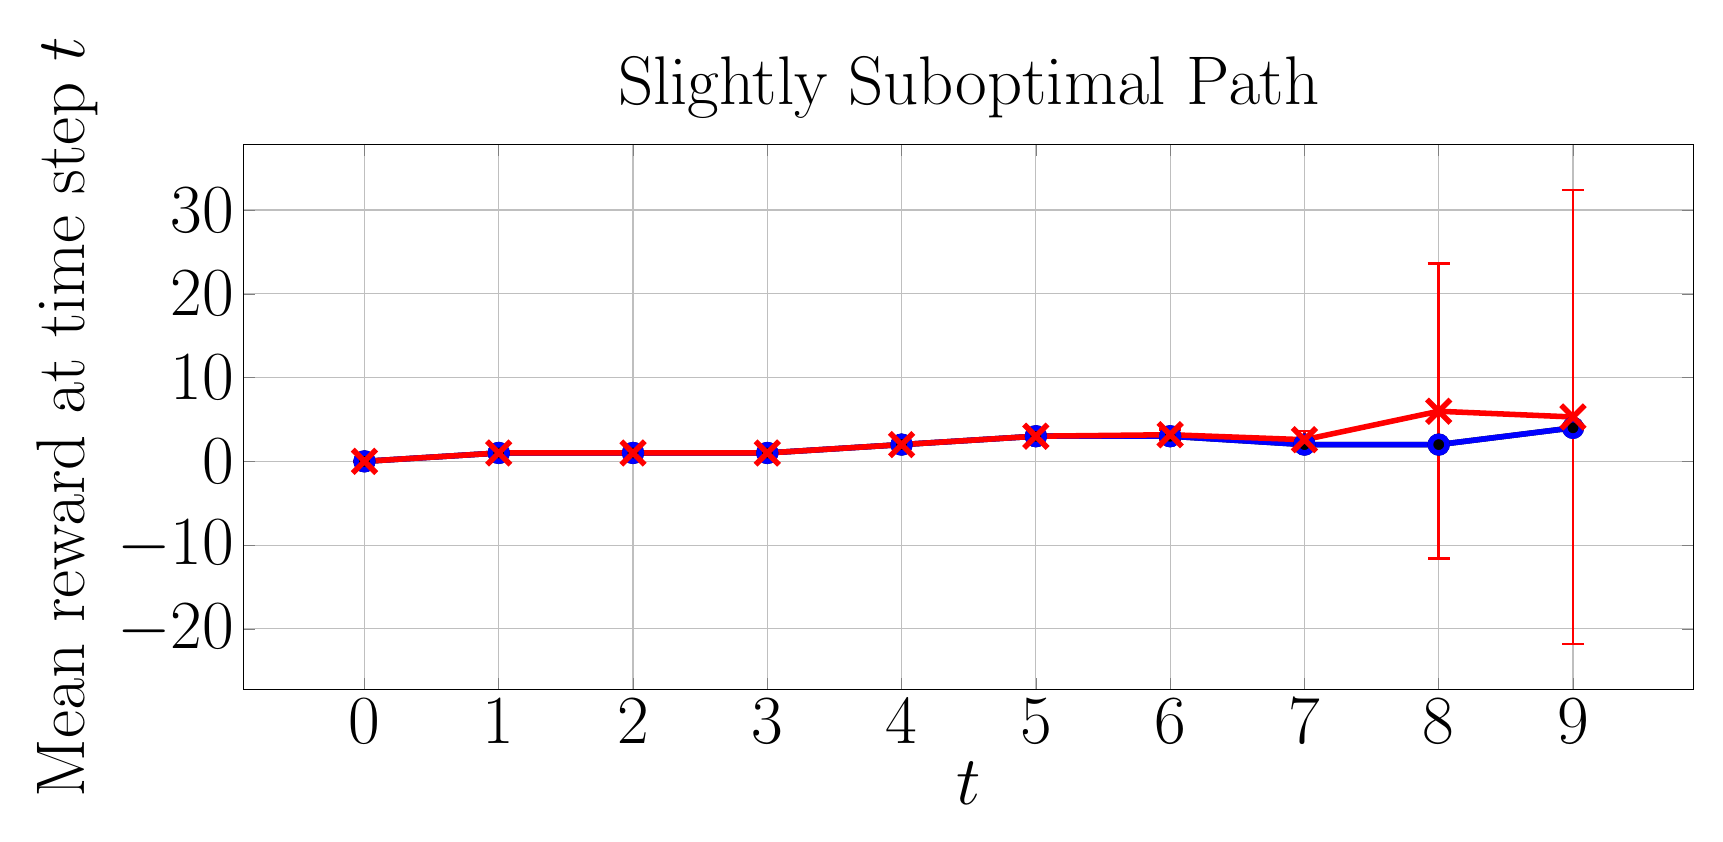
\begin{tikzpicture}
                \begin{axis}[
                    xlabel={$t$},
                    ylabel={Mean reward at time step $t$},
                    title={Slightly Suboptimal Path},
                    grid=both,
                    width=20cm, height=8.5cm,
                    every axis/.style={font=\Huge},
                    %
                ]
                \addplot[
                    color=black, %
                    mark=*, %
                    line width=2pt,
                    mark size=3pt,
                    error bars/.cd,
                    y dir=both, %
                    y explicit, %
                    error bar style={line width=1pt,solid},
                    error mark options={line width=1pt,mark size=4pt,rotate=90}
                ]
              coordinates {
                    (0, 0.0)  +- (0, 0.0)
                    (1, 1.0)  +- (0, 0.0) 
                    (2, 1.0)  +- (0, 0.0) 
                    (3, 1.0)  +- (0, 0.0)
                    (4, 2.0)  +- (0, 0.0)
                    (5, 3.0) +- (0, 0.0)
                    (6, 3.0) +- (0, 0.0)
                    (7, 2.0) +- (0, 0.0)
                    (8, 2.0) +- (0, 0.0)
                    (9, 4.0) +- (0, 0.0)
                };
                %
                \addplot[
                    color=blue, %
                    mark=o, %
                    line width=2pt,
                    mark size=3pt,
                    error bars/.cd,
                    y dir=both, %
                    y explicit, %
                    error bar style={line width=1pt,solid},
                    error mark options={line width=1pt,mark size=4pt,rotate=90}
                ]
              coordinates {
                    (0, 0.0)  +- (0, 0.0)
                    (1, 1.0)  +- (0, 0.0) 
                    (2, 1.0)  +- (0, 0.0) 
                    (3, 1.0)  +- (0, 0.0)
                    (4, 2.0)  +- (0, 0.0)
                    (5, 3.0) +- (0, 0.0)
                    (6, 3.0) +- (0, 0.0)
                    (7, 2.0) +- (0, 0.0)
                    (8, 2.0) +- (0, 0.0)
                    (9, 4.0) +- (0, 0.0)
                };
                %
                \addplot[
                    color=red, %
                    mark=x, %
                    line width=2pt,
                    mark size=6pt,
                    error bars/.cd,
                    y dir=both, %
                    y explicit, %
                    error bar style={line width=1pt,solid},
                    error mark options={line width=1pt,mark size=4pt,rotate=90}
                ]
                coordinates {
                    (0, 0.0)  +- (0, 0.0)
                    (1, 1.0)  +- (0, 0.0) 
                    (2, 1.0)  +- (0, 0.0) 
                    (3, 1.0)  +- (0, 0.0)
                    (4, 2.0)  += (0, 0.0)
                    (5, 3.0)  += (0, 0.0)
                    (6, 3.17847) += (0, 0.62606746) -= (0, 0.62606746)
                    (7, 2.5832885) += (0, 1.04598233) -= (0, 1.04598233)
                    (8, 5.978909) += (0, 17.60137623) -= (0, 17.60137623)
                    (9, 5.297059) += (0, 27.09227512) -= (0, 27.09227512)
                };
                \end{axis}
            \end{tikzpicture}
         }
    }\\[-1.5pt]
    \subfigure[\footnotesize Lowest cumulative reward: Interval CFMDP ($14$), Gumbel-max SCM ($-598$)]{%
         \resizebox{0.76\columnwidth}{!}{
             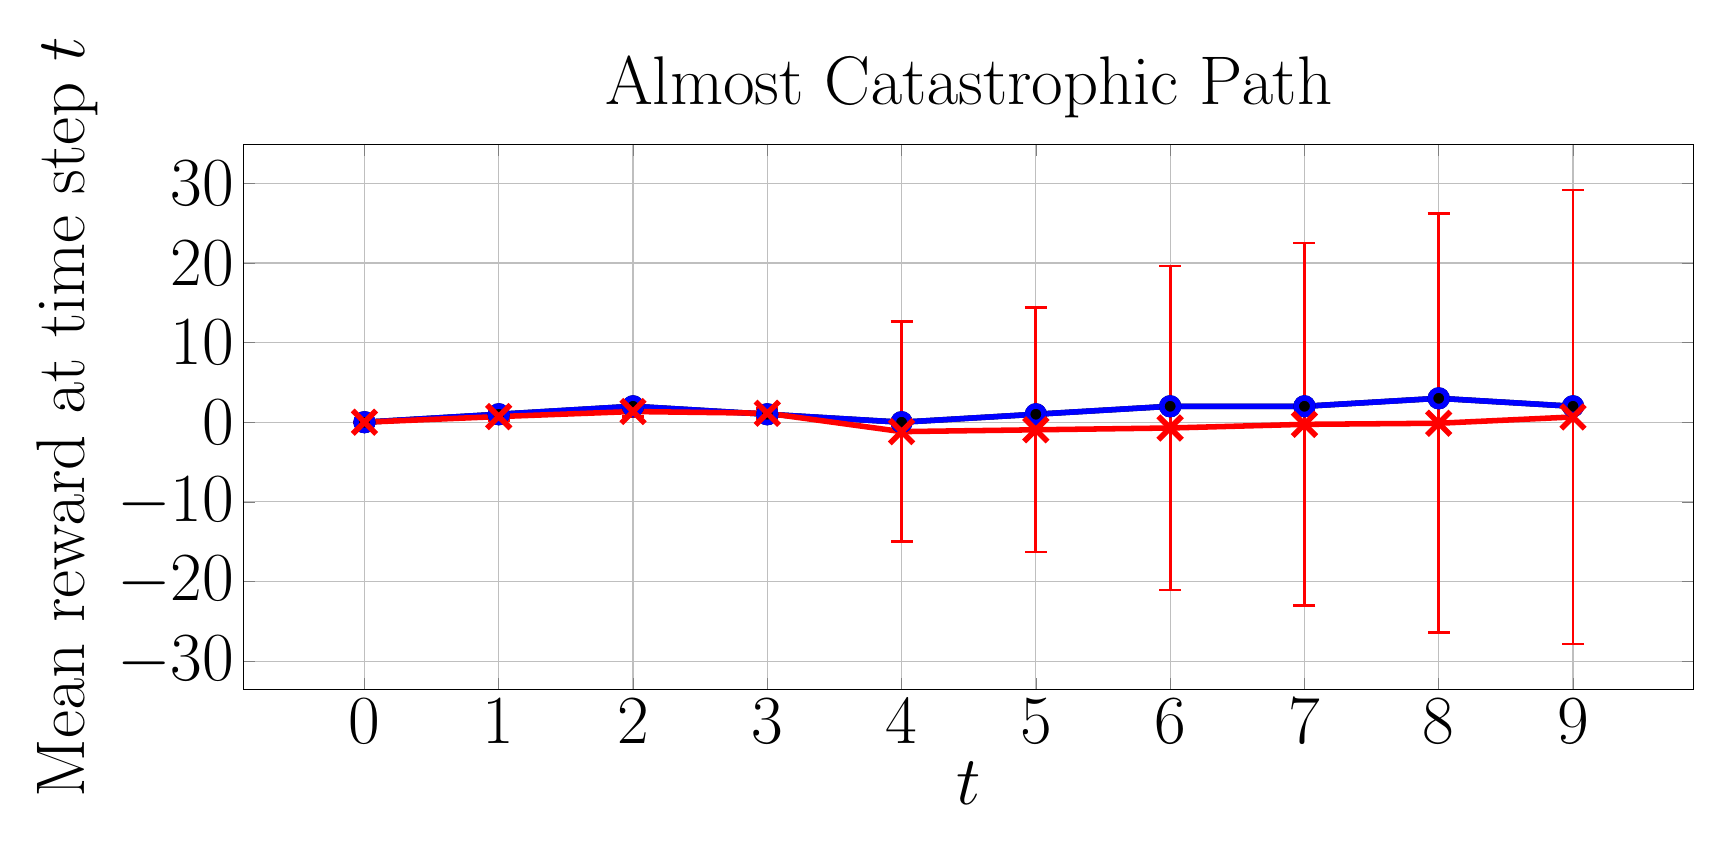
\begin{tikzpicture}
                \begin{axis}[
                    xlabel={$t$},
                    ylabel={Mean reward at time step $t$},
                    title={Almost Catastrophic Path},
                    grid=both,
                    width=20cm, height=8.5cm,
                    every axis/.style={font=\Huge},
                    %
                ]
                \addplot[
                    color=black, %
                    mark=*, %
                    line width=2pt,
                    mark size=3pt,
                    error bars/.cd,
                    y dir=both, %
                    y explicit, %
                    error bar style={line width=1pt,solid},
                    error mark options={line width=1pt,mark size=4pt,rotate=90}
                ]
                coordinates {
                    (0, 0.0)  +- (0, 0.0)
                    (1, 1.0)  +- (0, 0.0) 
                    (2, 2.0)  +- (0, 0.0) 
                    (3, 1.0)  +- (0, 0.0)
                    (4, 0.0)  +- (0, 0.0)
                    (5, 1.0) +- (0, 0.0)
                    (6, 2.0) +- (0, 0.0)
                    (7, 2.0) +- (0, 0.0)
                    (8, 3.0) +- (0, 0.0)
                    (9, 2.0) +- (0, 0.0)
                };
                %
                \addplot[
                    color=blue, %
                    mark=o, %
                    line width=2pt,
                    mark size=3pt,
                    error bars/.cd,
                    y dir=both, %
                    y explicit, %
                    error bar style={line width=1pt,solid},
                    error mark options={line width=1pt,mark size=4pt,rotate=90}
                ]
                coordinates {
                    (0, 0.0)  +- (0, 0.0)
                    (1, 1.0)  +- (0, 0.0) 
                    (2, 2.0)  +- (0, 0.0) 
                    (3, 1.0)  +- (0, 0.0)
                    (4, 0.0)  +- (0, 0.0)
                    (5, 1.0) +- (0, 0.0)
                    (6, 2.0) +- (0, 0.0)
                    (7, 2.0) +- (0, 0.0)
                    (8, 3.0) +- (0, 0.0)
                    (9, 2.0) +- (0, 0.0)
                };
                %
                \addplot[
                    color=red, %
                    mark=x, %
                    line width=2pt,
                    mark size=6pt,
                    error bars/.cd,
                    y dir=both, %
                    y explicit, %
                    error bar style={line width=1pt,solid},
                    error mark options={line width=1pt,mark size=4pt,rotate=90}
                ]
                coordinates {
                    (0, 0.0)  +- (0, 0.0)
                    (1, 0.7065655)  +- (0, 0.4553358) 
                    (2, 1.341673)  +- (0, 0.67091621) 
                    (3, 1.122926)  +- (0, 0.61281824)
                    (4, -1.1821935)  +- (0, 13.82444042)
                    (5, -0.952399)  +- (0, 15.35195457)
                    (6, -0.72672) +- (0, 20.33508414)
                    (7, -0.268983) +- (0, 22.77861454)
                    (8, -0.1310835) +- (0, 26.31013314)
                    (9, 0.65806) +- (0, 28.50670214)
                };
                %
            %
            %
            %
            %
            %
            %
            %
            %
            %
            %
            %
            %
            %
            %
            %
            %
            %
            %
                \end{axis}
            \end{tikzpicture}
         }
    }
    \hspace{1cm}
    \subfigure[\footnotesize Lowest cumulative reward: Interval CFMDP ($-698$), Gumbel-max SCM ($-698$)]{%
         \resizebox{0.76\columnwidth}{!}{
            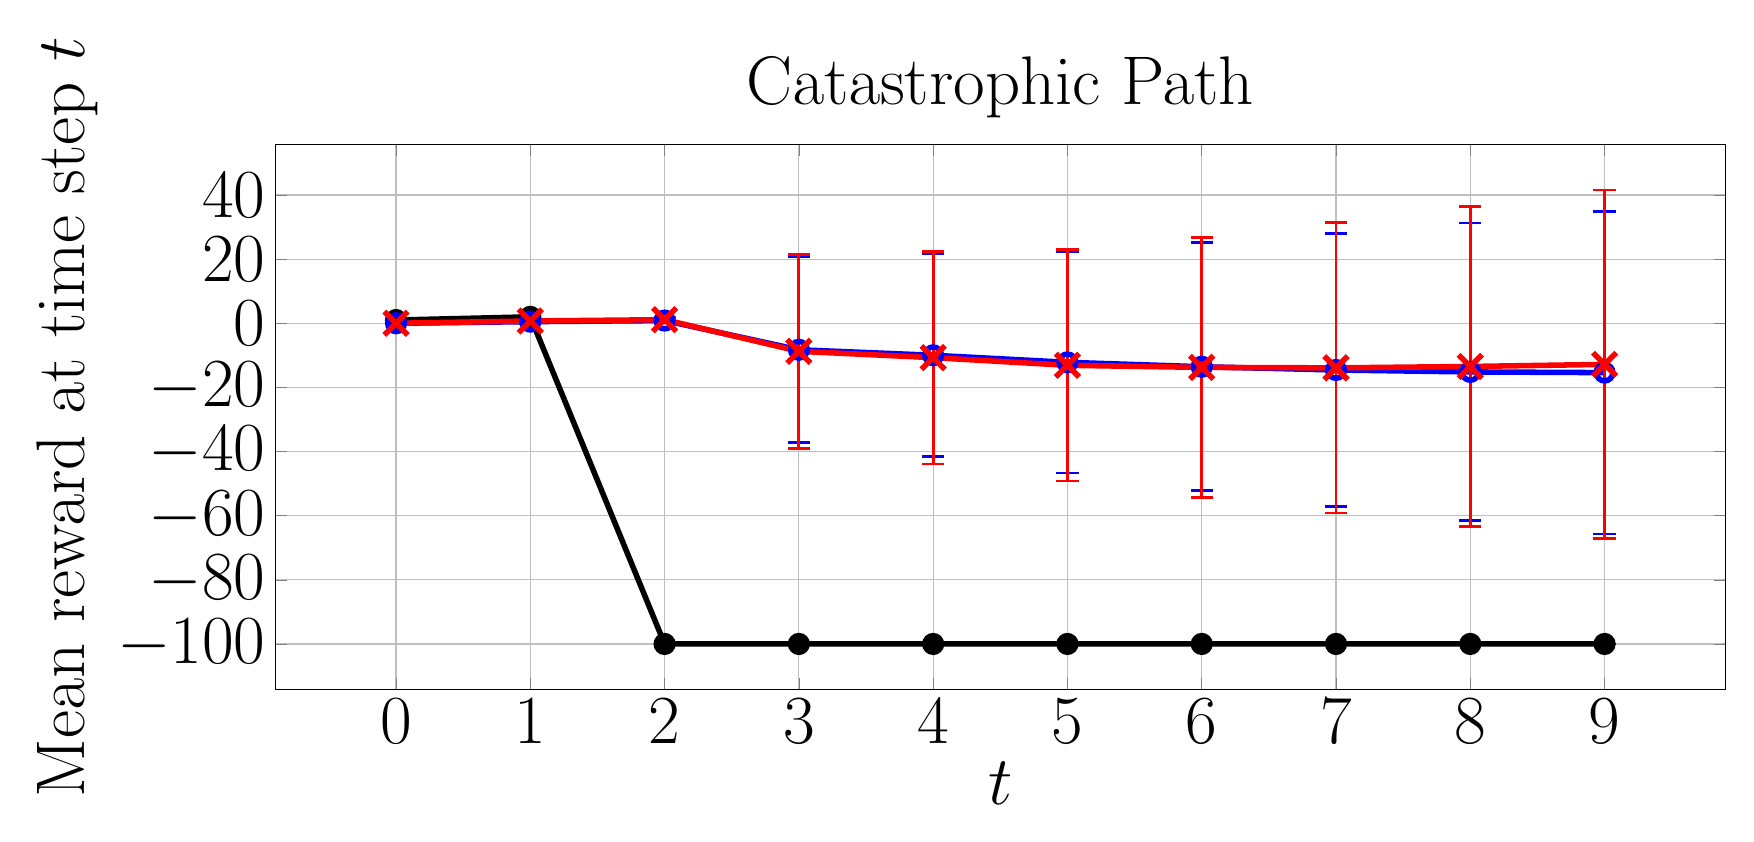
\begin{tikzpicture}
                \begin{axis}[
                    xlabel={$t$},
                    ylabel={Mean reward at time step $t$},
                    title={Catastrophic Path},
                    grid=both,
                    width=20cm, height=8.5cm,
                    every axis/.style={font=\Huge},
                    %
                ]
                \addplot[
                    color=black, %
                    mark=*, %
                    line width=2pt,
                    mark size=3pt,
                    error bars/.cd,
                    y dir=both, %
                    y explicit, %
                    error bar style={line width=1pt,solid},
                    error mark options={line width=1pt,mark size=4pt,rotate=90}
                ]
                coordinates {
                    (0, 1.0)  +- (0, 0.0)
                    (1, 2.0)  +- (0, 0.0) 
                    (2, -100.0)  +- (0, 0.0) 
                    (3, -100.0)  +- (0, 0.0)
                    (4, -100.0)  +- (0, 0.0)
                    (5, -100.0) +- (0, 0.0)
                    (6, -100.0) +- (0, 0.0)
                    (7, -100.0) +- (0, 0.0)
                    (8, -100.0) +- (0, 0.0)
                    (9, -100.0) +- (0, 0.0)
                };
                %
                \addplot[
                    color=blue, %
                    mark=o, %
                    line width=2pt,
                    mark size=3pt,
                    error bars/.cd,
                    y dir=both, %
                    y explicit, %
                    error bar style={line width=1pt,solid},
                    error mark options={line width=1pt,mark size=4pt,rotate=90}
                ]
                coordinates {
                    (0, 0.0)  +- (0, 0.0)
                    (1, 0.504814)  +- (0, 0.49997682) 
                    (2, 0.8439835)  +- (0, 0.76831917) 
                    (3, -8.2709165)  +- (0, 28.93656754)
                    (4, -9.981082)  +- (0, 31.66825363)
                    (5, -12.1776325) +- (0, 34.53463233)
                    (6, -13.556076) +- (0, 38.62845372)
                    (7, -14.574418) +- (0, 42.49603359)
                    (8, -15.1757075) +- (0, 46.41913968)
                    (9, -15.3900395) +- (0, 50.33563368)
                };
                %
                \addplot[
                    color=red, %
                    mark=x, %
                    line width=2pt,
                    mark size=6pt,
                    error bars/.cd,
                    y dir=both, %
                    y explicit, %
                    error bar style={line width=1pt,solid},
                    error mark options={line width=1pt,mark size=4pt,rotate=90}
                ]
                coordinates {
                    (0, 0.0)  +- (0, 0.0)
                    (1, 0.701873)  +- (0, 0.45743556) 
                    (2, 1.1227805)  +- (0, 0.73433129) 
                    (3, -8.7503255)  +- (0, 30.30257976)
                    (4, -10.722092)  +- (0, 33.17618589)
                    (5, -13.10721)  +- (0, 36.0648089)
                    (6, -13.7631645) +- (0, 40.56553451)
                    (7, -13.909043) +- (0, 45.23829402)
                    (8, -13.472517) +- (0, 49.96270296)
                    (9, -12.8278835) +- (0, 54.38618735)
                };
                %
            %
            %
            %
            %
            %
            %
            %
            %
            %
            %
            %
            %
            %
            %
            %
            %
            %
            %
                \end{axis}
            \end{tikzpicture}
         }
    }
    \caption{Average instant reward of CF paths induced by policies on GridWorld $p=0.4$.}
    \label{fig: reward p=0.4}
\end{figure*}

\subsection{Experimental Setup}
To compare policy performance, we measure the average rewards of counterfactual paths induced by our policy and the Gumbel-max policy by uniformly sampling $200$ counterfactual MDPs from the ICFMDP and generating $10,000$ counterfactual paths over each sampled CFMDP. \jl{Since the interval CFMDP depends on the observed path, we select $4$  paths of varying optimality to evaluate how the observed path impacts the performance of both policies: an optimal path, a slightly suboptimal path that could reach the optimal reward with a few changes, a catastrophic path that enters a catastrophic, terminal state with low reward, and an almost catastrophic path that was close to entering a catastrophic state.} When measuring the average probability bound widths and execution time needed to generate the ICFMDPs, we averaged over $20$ randomly generated observed paths
\footnote{Further training details are provided in Appendix \ref{app: training details}, and the code is provided at \href{https://github.com/ddv-lab/robust-cf-inference-in-MDPs}{https://github.com/ddv-lab/robust-cf-inference-in-MDPs}
%
%
.}.

\subsection{GridWorld}
\jl{The GridWorld MDP is a $4 \times 4$ grid where an agent must navigate from the top-left corner to the goal state in the bottom-right corner, avoiding a dangerous terminal state in the centre. At each time step, the agent can move up, down, left, or right, but there is a small probability (controlled by hyper-parameter $p$) of moving in an unintended direction. As the agent nears the goal, the reward for each state increases, culminating in a reward of $+100$ for reaching the goal. Entering the dangerous state results in a penalty of $-100$. We use two versions of GridWorld: a less stochastic version with $p=0.9$ (i.e., $90$\% chance of moving in the chosen direction) and a more stochastic version with $p=0.4$.}

\paragraph{GridWorld ($p=0.9$)}
When $p=0.9$, the counterfactual probability bounds are typically narrow (see Table \ref{tab:nonzero_probs} for average measurements). Consequently, as shown in Figure \ref{fig: reward p=0.9}, both policies are nearly identical and perform similarly well across the optimal, slightly suboptimal, and catastrophic paths.
%
However, for the almost catastrophic path, the interval CFMDP path is more conservative and follows the observed path more closely (as this is where the probability bounds are narrowest), which typically requires one additional step to reach the goal state than the Gumbel-max SCM policy.
%

\paragraph{GridWorld ($p=0.4$)}
\jl{When $p=0.4$, the GridWorld environment becomes more uncertain, increasing the risk of entering the dangerous state even if correct actions are chosen. Thus, as shown in Figure \ref{fig: reward p=0.4}, the interval CFMDP policy adopts a more conservative approach, avoiding deviation from the observed policy if it cannot guarantee higher counterfactual rewards (see the slightly suboptimal and almost catastrophic paths), whereas the Gumbel-max SCM is inconsistent: it can yield higher rewards, but also much lower rewards, reflected in the wide error bars.} For the catastrophic path, both policies must deviate from the observed path to achieve a higher reward and, in this case, perform similarly.
%
%
%
%
\subsection{Sepsis}
The Sepsis MDP \citep{oberst2019counterfactual} simulates trajectories of Sepsis patients. Each state consists of four vital signs (heart rate, blood pressure, oxygen concentration, and glucose levels), categorised as low, normal, or high.
and three treatments that can be toggled on/off at each time step (8 actions in total). Unlike \citet{oberst2019counterfactual}, we scale rewards based on the number of out-of-range vital signs, between $-1000$ (patient dies) and $1000$ (patient discharged). \jl{Like the GridWorld $p=0.4$ experiment, the Sepsis MDP is highly uncertain, as many states are equally likely to lead to optimal and poor outcomes. Thus, as shown in Figure \ref{fig: reward sepsis}, both policies follow the observed optimal and almost catastrophic paths to guarantee rewards are no worse than the observation.} However, improving the catastrophic path requires deviating from the observation. Here, the Gumbel-max SCM policy, on average, performs better than the interval CFMDP policy. But, since both policies have lower bounds clipped at $-1000$, neither policy reliably improves over the observation. In contrast, for the slightly suboptimal path, the interval CFMDP policy performs significantly better, shown by its higher lower bounds. 
Moreover, in these two cases, the worst-case counterfactual path generated by the interval CFMDP policy is better than that of the Gumbel-max SCM policy,
indicating its greater robustness.
%
\begin{figure*}
    \centering
     \resizebox{0.6\textwidth}{!}{
        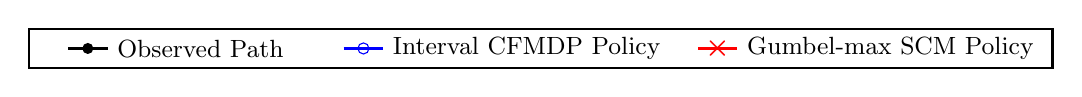
\begin{tikzpicture}[scale=1.0, every node/.style={scale=1.0}]
            \draw[thick, black] (-3, -0.25) rectangle (10, 0.25);
            %
            \draw[black, line width=1pt] (-2.5, 0.0) -- (-2,0.0);
            \fill[black] (-2.25,0.0) circle (2pt); %
            \node[right] at (-2,0.0) {\small Observed Path};
            
            %
            \draw[blue, line width=1pt] (1.0,0.0) -- (1.5,0.0);
            \node[draw=blue, circle, minimum size=4pt, inner sep=0pt] at (1.25,0.0) {}; %
            \node[right] at (1.5,0.0) {\small Interval CFMDP Policy};
            
            %
            \draw[red, line width=1pt] (5.5,0) -- (6,0);
            \node[red] at (5.75,0) {$\boldsymbol{\times}$}; %
            \node[right] at (6,0) {\small Gumbel-max SCM Policy};
        \end{tikzpicture}
    }\\
    \subfigure[\footnotesize Lowest cumulative reward: Interval CFMDP ($8000$), Gumbel-max SCM ($8000$)]{%
         \resizebox{0.76\columnwidth}{!}{
             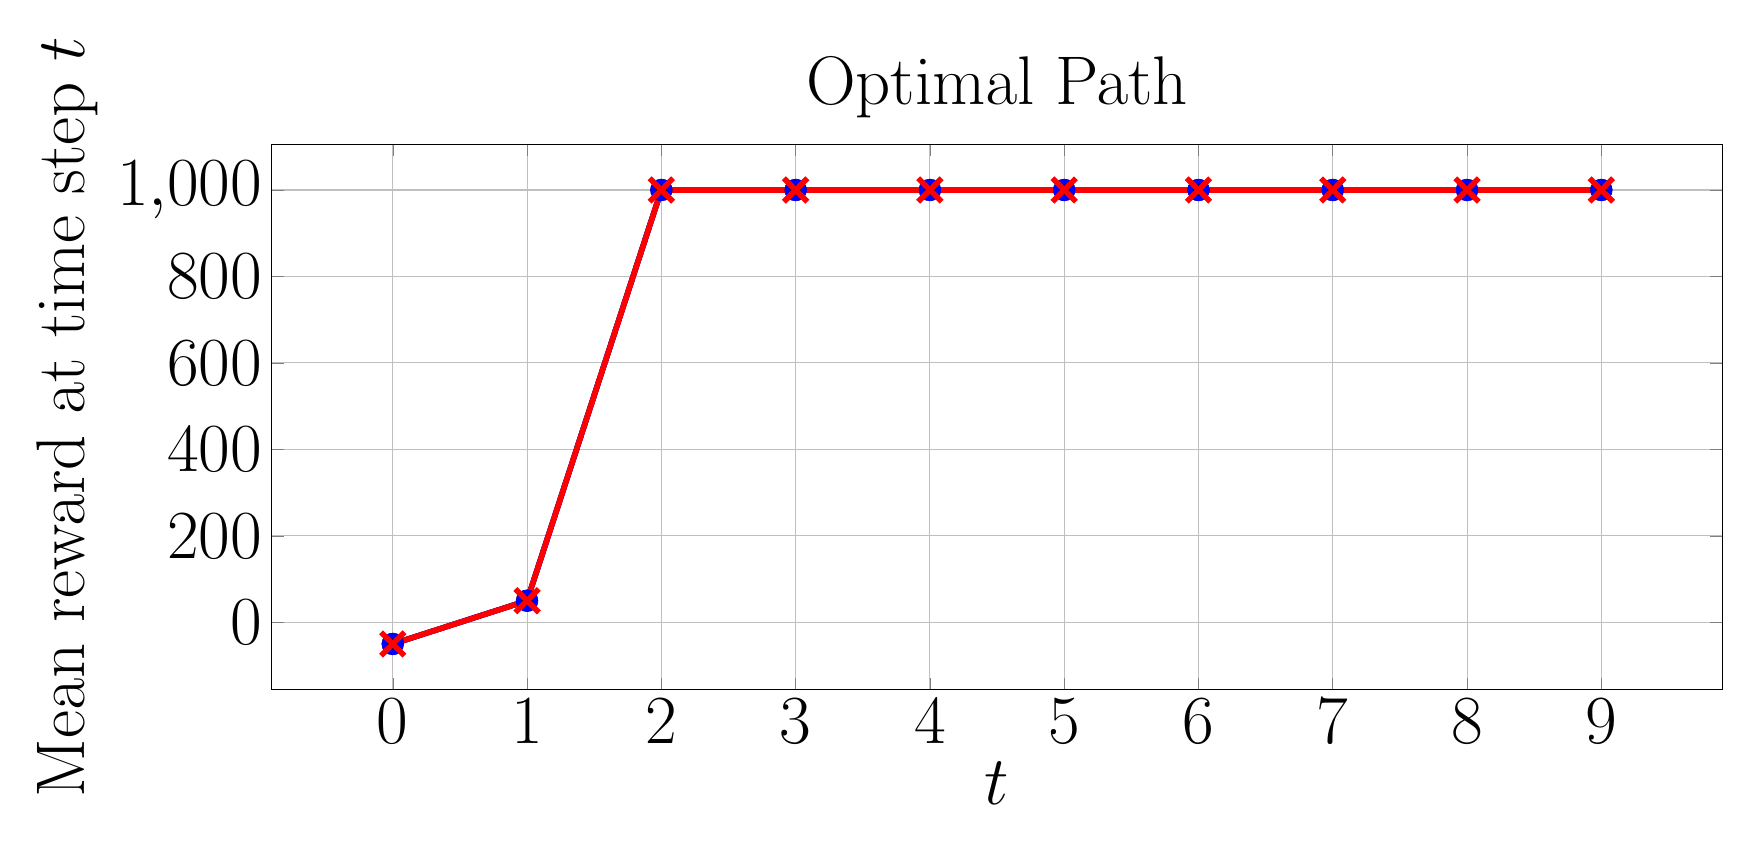
\begin{tikzpicture}
                \begin{axis}[
                    xlabel={$t$},
                    ylabel={Mean reward at time step $t$},
                    title={Optimal Path},
                    grid=both,
                    width=20cm, height=8.5cm,
                    every axis/.style={font=\Huge},
                    %
                ]
                \addplot[
                    color=black, %
                    mark=*, %
                    line width=2pt,
                    mark size=3pt,
                ]
                coordinates {
                    (0, -50.0)
                    (1, 50.0)
                    (2, 1000.0)
                    (3, 1000.0)
                    (4, 1000.0)
                    (5, 1000.0)
                    (6, 1000.0)
                    (7, 1000.0)
                    (8, 1000.0)
                    (9, 1000.0)
                };
                %
                \addplot[
                    color=blue, %
                    mark=o, %
                    line width=2pt,
                    mark size=3pt,
                    error bars/.cd,
                    y dir=both, %
                    y explicit, %
                    error bar style={line width=1pt,solid},
                    error mark options={line width=1pt,mark size=4pt,rotate=90}
                ]
                coordinates {
                    (0, -50.0)  +- (0, 0.0)
                    (1, 50.0)  +- (0, 0.0) 
                    (2, 1000.0)  +- (0, 0.0) 
                    (3, 1000.0)  +- (0, 0.0)
                    (4, 1000.0)  +- (0, 0.0)
                    (5, 1000.0) +- (0, 0.0)
                    (6, 1000.0) +- (0, 0.0)
                    (7, 1000.0) +- (0, 0.0)
                    (8, 1000.0) +- (0, 0.0)
                    (9, 1000.0) +- (0, 0.0)
                };
                %
                \addplot[
                    color=red, %
                    mark=x, %
                    line width=2pt,
                    mark size=6pt,
                    error bars/.cd,
                    y dir=both, %
                    y explicit, %
                    error bar style={line width=1pt,solid},
                    error mark options={line width=1pt,mark size=4pt,rotate=90}
                ]
                coordinates {
                    (0, -50.0)  +- (0, 0.0)
                    (1, 50.0)  +- (0, 0.0) 
                    (2, 1000.0)  +- (0, 0.0) 
                    (3, 1000.0)  +- (0, 0.0)
                    (4, 1000.0)  +- (0, 0.0)
                    (5, 1000.0) +- (0, 0.0)
                    (6, 1000.0) +- (0, 0.0)
                    (7, 1000.0) +- (0, 0.0)
                    (8, 1000.0) +- (0, 0.0)
                    (9, 1000.0) +- (0, 0.0)
                };
                %
                \end{axis}
            \end{tikzpicture}
         }
    }
    \hspace{1cm}
    \subfigure[\footnotesize Lowest cumulative reward: Interval CFMDP ($-5980$), Gumbel-max SCM ($-8000$)]{%
         \resizebox{0.76\columnwidth}{!}{
            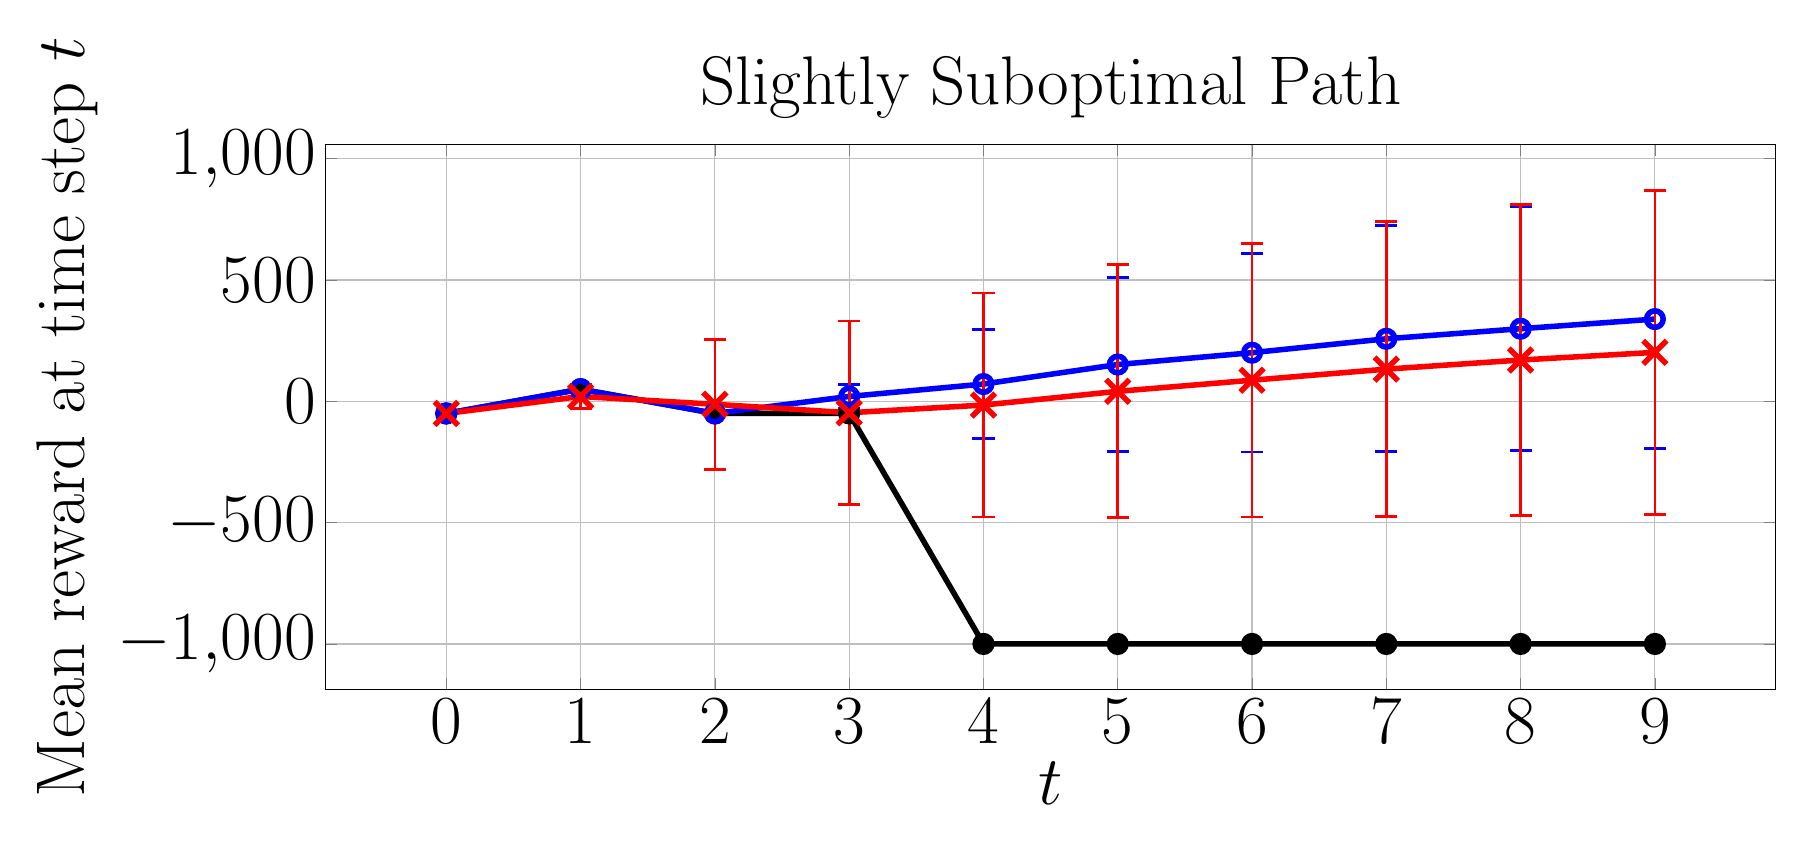
\begin{tikzpicture}
                \begin{axis}[
                    xlabel={$t$},
                    ylabel={Mean reward at time step $t$},
                    title={Slightly Suboptimal Path},
                    grid=both,
                    width=20cm, height=8.5cm,
                    every axis/.style={font=\Huge},
                    %
                ]
               \addplot[
                    color=black, %
                    mark=*, %
                    line width=2pt,
                    mark size=3pt,
                ]
                coordinates {
                    (0, -50.0)
                    (1, 50.0)
                    (2, -50.0)
                    (3, -50.0)
                    (4, -1000.0)
                    (5, -1000.0)
                    (6, -1000.0)
                    (7, -1000.0)
                    (8, -1000.0)
                    (9, -1000.0)
                };
                %
                \addplot[
                    color=blue, %
                    mark=o, %
                    line width=2pt,
                    mark size=3pt,
                    error bars/.cd,
                    y dir=both, %
                    y explicit, %
                    error bar style={line width=1pt,solid},
                    error mark options={line width=1pt,mark size=4pt,rotate=90}
                ]
                coordinates {
                    (0, -50.0)  +- (0, 0.0)
                    (1, 50.0)  +- (0, 0.0) 
                    (2, -50.0)  +- (0, 0.0) 
                    (3, 20.0631)  +- (0, 49.97539413)
                    (4, 71.206585)  +- (0, 226.02033693)
                    (5, 151.60797) +- (0, 359.23292559)
                    (6, 200.40593) +- (0, 408.86185176)
                    (7, 257.77948) +- (0, 466.10372804)
                    (8, 299.237465) +- (0, 501.82579506)
                    (9, 338.9129) +- (0, 532.06124996)
                };
                %
                \addplot[
                    color=red, %
                    mark=x, %
                    line width=2pt,
                    mark size=6pt,
                    error bars/.cd,
                    y dir=both, %
                    y explicit, %
                    error bar style={line width=1pt,solid},
                    error mark options={line width=1pt,mark size=4pt,rotate=90}
                ]
                coordinates {
                    (0, -50.0)  +- (0, 0.0)
                    (1, 20.00736)  +- (0, 49.99786741) 
                    (2, -12.282865)  +- (0, 267.598755) 
                    (3, -47.125995)  +- (0, 378.41755832)
                    (4, -15.381965)  +- (0, 461.77616558)
                    (5, 41.15459) +- (0, 521.53189262)
                    (6, 87.01595) +- (0, 564.22243126 )
                    (7, 132.62376) +- (0, 607.31338037)
                    (8, 170.168145) +- (0, 641.48013693)
                    (9, 201.813135) +- (0, 667.29441777)
                };
                %
                %
                %
                %
                %
                %
                %
                %
                %
                %
                %
                %
                %
                %
                %
                %
                %
                %
                %
                \end{axis}
            \end{tikzpicture}
         }
    }\\[-1.5pt]
    \subfigure[\footnotesize Lowest cumulative reward: Interval CFMDP ($100$), Gumbel-max SCM ($100$)]{%
         \resizebox{0.76\columnwidth}{!}{
             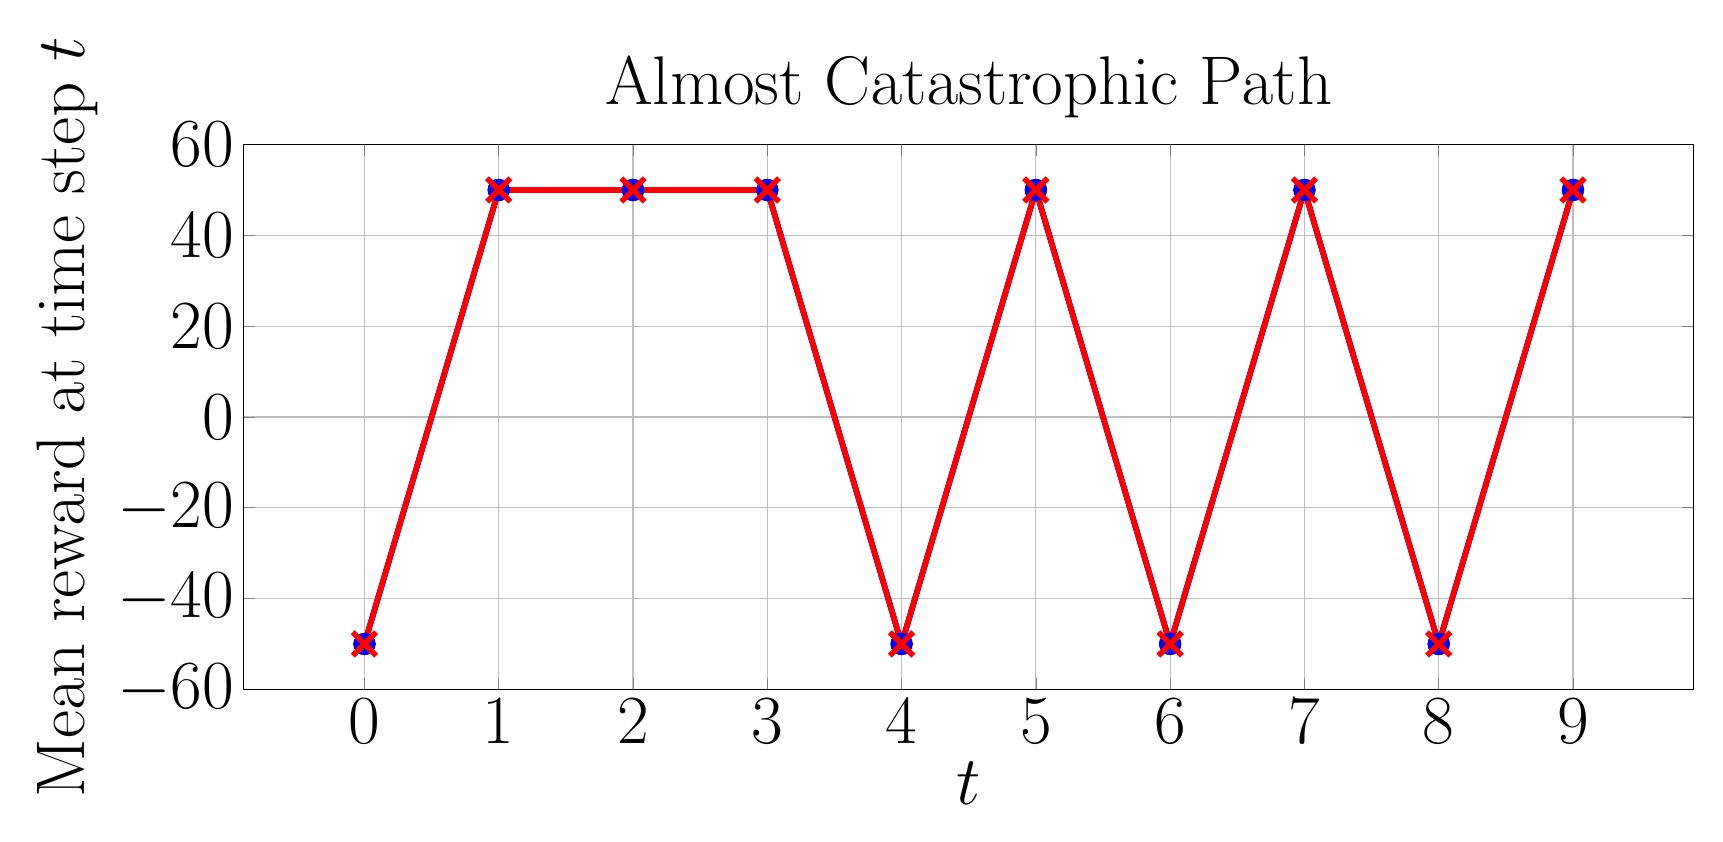
\begin{tikzpicture}
                \begin{axis}[
                    xlabel={$t$},
                    ylabel={Mean reward at time step $t$},
                    title={Almost Catastrophic Path},
                    grid=both,
                    every axis/.style={font=\Huge},
                    width=20cm, height=8.5cm,
                    %
                ]
               \addplot[
                    color=black, %
                    mark=*, %
                    line width=2pt,
                    mark size=3pt,
                ]
                coordinates {
                    (0, -50.0)
                    (1, 50.0)
                    (2, 50.0)
                    (3, 50.0)
                    (4, -50.0)
                    (5, 50.0)
                    (6, -50.0)
                    (7, 50.0)
                    (8, -50.0)
                    (9, 50.0)
                };
                %
                %
                \addplot[
                    color=blue, %
                    mark=o, %
                    line width=2pt,
                    mark size=3pt,
                    error bars/.cd,
                    y dir=both, %
                    y explicit, %
                    error bar style={line width=1pt,solid},
                    error mark options={line width=1pt,mark size=4pt,rotate=90}
                ]
                coordinates {
                    (0, -50.0)  +- (0, 0.0)
                    (1, 50.0)  +- (0, 0.0) 
                    (2, 50.0)  +- (0, 0.0) 
                    (3, 50.0)  +- (0, 0.0)
                    (4, -50.0)  +- (0, 0.0)
                    (5, 50.0) +- (0, 0.0)
                    (6, -50.0) +- (0, 0.0)
                    (7, 50.0) +- (0, 0.0)
                    (8, -50.0) +- (0, 0.0)
                    (9, 50.0) +- (0, 0.0)
                };
                %
                \addplot[
                    color=red, %
                    mark=x, %
                    line width=2pt,
                    mark size=6pt,
                    error bars/.cd,
                    y dir=both, %
                    y explicit, %
                    error bar style={line width=1pt,solid},
                    error mark options={line width=1pt,mark size=4pt,rotate=90}
                ]
                coordinates {
                    (0, -50.0)  +- (0, 0.0)
                    (1, 50.0)  +- (0, 0.0) 
                    (2, 50.0)  +- (0, 0.0) 
                    (3, 50.0)  +- (0, 0.0)
                    (4, -50.0)  +- (0, 0.0)
                    (5, 50.0) +- (0, 0.0)
                    (6, -50.0) +- (0, 0.0)
                    (7, 50.0) +- (0, 0.0)
                    (8, -50.0) +- (0, 0.0)
                    (9, 50.0) +- (0, 0.0)
                };
                %
                %
                %
                %
                %
                %
                %
                %
                %
                %
                %
                %
                %
                %
                %
                %
                %
                %
                %
                \end{axis}
            \end{tikzpicture}
         }
    }
    \hspace{1cm}
    \subfigure[\footnotesize Lowest cumulative reward: Interval CFMDP ($-7150$), Gumbel-max SCM ($-9050$)]{%
         \resizebox{0.76\columnwidth}{!}{
            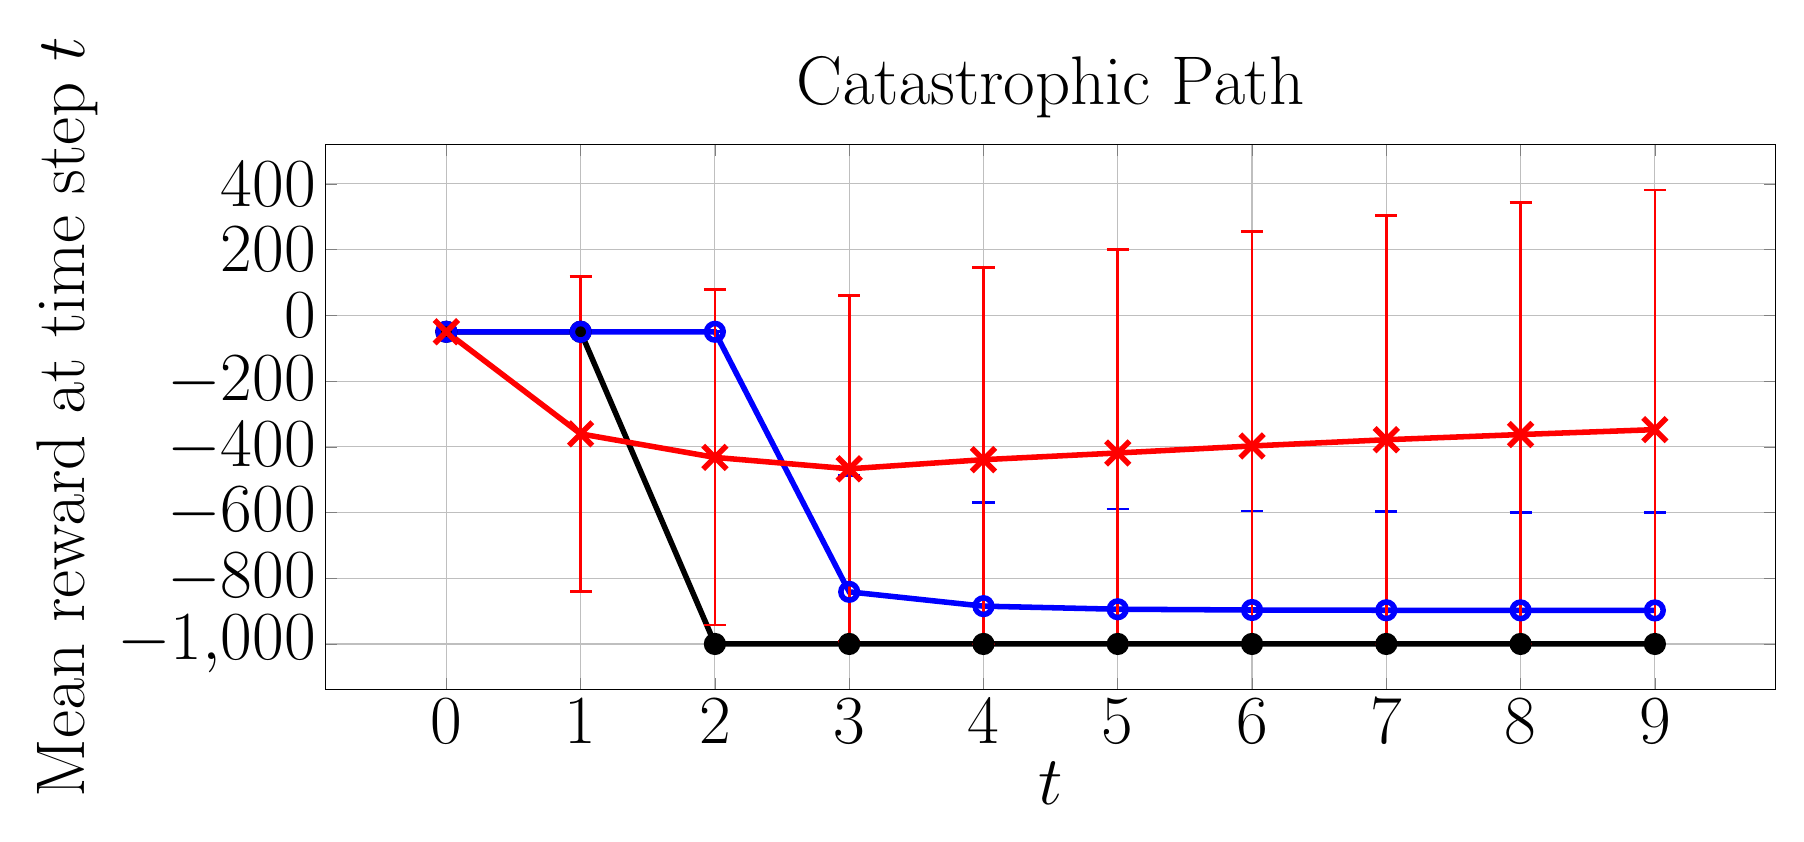
\begin{tikzpicture}
                \begin{axis}[
                    xlabel={$t$},
                    ylabel={Mean reward at time step $t$},
                    title={Catastrophic Path},
                    grid=both,
                    width=20cm, height=8.5cm,
                    every axis/.style={font=\Huge},
                    %
                ]
               \addplot[
                    color=black, %
                    mark=*, %
                    line width=2pt,
                    mark size=3pt,
                ]
                coordinates {
                    (0, -50.0)
                    (1, -50.0)
                    (2, -1000.0)
                    (3, -1000.0)
                    (4, -1000.0)
                    (5, -1000.0)
                    (6, -1000.0)
                    (7, -1000.0)
                    (8, -1000.0)
                    (9, -1000.0)
                };
                %
                %
                \addplot[
                    color=blue, %
                    mark=o, %
                    line width=2pt,
                    mark size=3pt,
                    error bars/.cd,
                    y dir=both, %
                    y explicit, %
                    error bar style={line width=1pt,solid},
                    error mark options={line width=1pt,mark size=4pt,rotate=90}
                ]
                coordinates {
                    (0, -50.0)  +- (0, 0.0)
                    (1, -50.0)  +- (0, 0.0) 
                    (2, -50.0)  +- (0, 0.0) 
                    (3, -841.440725)  += (0, 354.24605512) -= (0, 158.559275)
                    (4, -884.98225)  += (0, 315.37519669) -= (0, 115.01775)
                    (5, -894.330425) += (0, 304.88572805) -= (0, 105.669575)
                    (6, -896.696175) += (0, 301.19954514) -= (0, 103.303825)
                    (7, -897.4635) += (0, 299.61791279) -= (0, 102.5365)
                    (8, -897.77595) += (0, 298.80392585) -= (0, 102.22405)
                    (9, -897.942975) += (0, 298.32920557) -= (0, 102.057025)
                };
                %
                \addplot[
                    color=red, %
                    mark=x, %
                    line width=2pt,
                    mark size=6pt,
                    error bars/.cd,
                    y dir=both, %
                    y explicit, %
                    error bar style={line width=1pt,solid},
                    error mark options={line width=1pt,mark size=4pt,rotate=90}
                ]
            coordinates {
                    (0, -50.0)  +- (0, 0.0)
                    (1, -360.675265)  +- (0, 479.39812699) 
                    (2, -432.27629)  +- (0, 510.38620897) 
                    (3, -467.029545)  += (0, 526.36009628) -= (0, 526.36009628)
                    (4, -439.17429)  += (0, 583.96638919) -= (0, 560.82571)
                    (5, -418.82704) += (0, 618.43027478) -= (0, 581.17296)
                    (6, -397.464895) += (0, 652.67322574) -= (0, 602.535105)
                    (7, -378.49052) += (0, 682.85407033) -= (0, 621.50948)
                    (8, -362.654195) += (0, 707.01412023) -= (0, 637.345805)
                    (9, -347.737935) += (0, 729.29076479) -= (0, 652.262065)
                };
                %
                %
                %
                %
                %
                %
                %
                %
                %
                %
                %
                %
                %
                %
                %
                %
                %
                %
                %
                \end{axis}
            \end{tikzpicture}
         }
    }
    \caption{Average instant reward of CF paths induced by policies on Sepsis.}
    \label{fig: reward sepsis}
\end{figure*}

%
%
%
\subsection{Interval CFMDP Bounds}
%
%
Table \ref{tab:nonzero_probs} presents the mean counterfactual probability bound widths (excluding transitions where the upper bound is $0$) for each MDP, averaged over 20 observed paths. We compare the bounds under counterfactual stability (CS) and monotonicity (M) assumptions, CS alone, and no assumptions. This shows that the assumptions marginally reduce the bound widths, indicating the assumptions tighten the bounds without excluding too many causal models, as intended.
\renewcommand{\arraystretch}{1}

\begin{table}
\centering
\caption{Mean width of counterfactual probability bounds}
\resizebox{0.8\columnwidth}{!}{%
\begin{tabular}{|c|c|c|c|}
\hline
\multirow{2}{*}{\textbf{Environment}} & \multicolumn{3}{c|}{\textbf{Assumptions}} \\ \cline{2-4}
 & \textbf{CS + M} & \textbf{CS} & \textbf{None\tablefootnote{\jl{Equivalent to \citet{li2024probabilities}'s bounds (see Section \ref{sec: equivalence with Li}).}}} \\ \hline
\textbf{GridWorld} ($p=0.9$) & 0.0817 & 0.0977 & 0.100 \\ \hline
\textbf{GridWorld} ($p=0.4$) & 0.552  & 0.638  & 0.646 \\ \hline
\textbf{Sepsis} & 0.138 & 0.140 & 0.140 \\ \hline
\end{tabular}
}
\label{tab:nonzero_probs}
\end{table}


\subsection{Execution Times}
Table \ref{tab: times} compares the average time needed to generate the interval CFMDP vs.\ the Gumbel-max SCM CFMDP for 20 observations.
The GridWorld algorithms were run single-threaded, while the Sepsis experiments were run in parallel.
Generating the interval CFMDP is significantly faster as it uses exact analytical bounds, whereas the Gumbel-max CFMDP requires sampling from the Gumbel distribution to estimate counterfactual transition probabilities. \jl{Since constructing the counterfactual MDP models is the main bottleneck in both approaches, ours is more efficient overall and suitable for larger MDPs.}
\begin{table}
\centering
\caption{Mean execution time to generate CFMDPs}
\resizebox{0.99\columnwidth}{!}{%
\begin{tabular}{|c|c|c|}
\hline
\multirow{2}{*}{\textbf{Environment}} & \multicolumn{2}{c|}{\textbf{Mean Execution Time (s)}} \\ \cline{2-3} 
                                      & \textbf{Interval CFMDP} & \textbf{Gumbel-max CFMDP} \\ \hline
\textbf{GridWorld ($p=0.9$) }                  & 0.261                   & 56.1                      \\ \hline
\textbf{GridWorld ($p=0.4$)  }                 & 0.336                   & 54.5                      \\ \hline
\textbf{Sepsis}                                 & 688                     & 2940                      \\ \hline
\end{tabular}%
}
\label{tab: times}
\end{table}


%Figure
\begin{figure*}[h]
    \vskip 0.2in
    \begin{center}
        \centerline{\includegraphics[width=\linewidth]{imgs/graphs/heatmap_all.png}}
        \caption{Cumulative heatmaps of VLMs' minimal paths to the goal state after 20 steps across varying complexities, with the number of geoms and shortest path solutions ranging from 2 to 11. Evaluated over 5400 episodes across all modalities (vision 3D, vision 2D, text).}
        \label{fig:cumulative_heatmap}
    \end{center}
    \vskip -0.2in
\end{figure*}

%%%%%%%%%%%%%%%%%%%%%%%%%%%%%%%%
% Results
%%%%%%%%%%%%%%%%%%%%%%%%%%%%%%%%
\section{Results}
\label{results}

%Footnote
%% TODO
% more detailed introduction of dataset creation
% the rumour label in such datasets
\section{Data} \label{sec:data}
We use three rumour datasets in this work, namely: PHEME~\citep{pheme2015,kochkina-etal-2018-one}, Twitter15, and Twitter16~\citep{ma-etal-2017-detect}:

% TJB: how can the number of threads be greater than the number of tweets? these numbers don't make sense
% RX: fixed, the numbers were incorrect
\paragraph{PHEME}~\citet{pheme2015} contains 6,425 tweet posts of rumours and non-rumours related to 9 events. To avoid using specific a priori keywords to search for tweet posts, PHEME used the Twitter (now X) steaming API to identify newsworthy events from breaking news and then selected from candidate rumours that met rumour criteria, finally they collected associated conversations and annotate them. They engaged journalists to annotate the threads. The data were collected between 2014 and 2015. The 9 events are split into two groups, the first being breaking news that contains rumours, including Ferguson unrest, Ottawa shooting, Sydney siege, Charlie Hebdo shooting, and Germanwings plane crash. The rest are specific rumours, namely Prince to play in Toronto, Gurlitt collection, Putin missing, and Michael Essien contracting Ebola.
% TJB: say something about the time period when this data was collected
% RX: added

\paragraph{Twitter 15}~\citet{twitter15} was constructed by collecting rumour and non-rumour posts from the tracking websites snopes.com and emergent.info. They then used the Twitter API to gather corresponding posts, resulting in 94 true and 446 false posts. This dataset further includes 1,490 root posts and their follow posts, comprising 1,116 rumours and 374 non-rumours.
% TJB: the "tweet" vs. "comment" terminology is potentially confusing and needs to be clarified
% RX: unified, used root and follow posts to refer to root posts and the comment posts, posts are used to describe tweets in general.

\paragraph{Twitter 16}
Similarly to Twitter 15, \citet{twitter16} collected rumours and non-rumours from snopes.com, resulting in 778 reported events, 64\% of which are rumours. For each event, keywords were extracted from the final part of the Snopes URL and refined manually---adding, deleting, or replacing words iteratively---until the composed queries yielded precise Twitter search results. The final dataset includes 1,490 root tweet posts and their follow posts, comprising 613 rumours and 205 non-rumours.

\begin{table*}[!t]
    \centering
    \small
    \begin{tabular}{p{0.05\linewidth}p{0.9\linewidth}}
    \toprule
    Task & Prompt \\
    \midrule
    V-oc & Categorize the text into an ordinal class that best characterizes the writer's mental state, considering various degrees of positive and negative sentiment intensity. 3: very positive mental state can be inferred. 2: moderately positive mental state can be inferred. 1: slightly positive mental state can be inferred. 0: neutral or mixed mental state can be inferred. -1: slightly negative mental state can be inferred. -2: moderately negative mental state can be inferred. -3: very negative mental state can be inferred.\\
    \midrule
    E-c & Categorize the text's emotional tone as either `neutral or no emotion' or identify the presence of one or more of the given emotions (anger, anticipation, disgust, fear, joy, love, optimism, pessimism, sadness, surprise, trust).\\
    \midrule
    E-i & Assign a numerical value between 0 (least E) and 1 (most E) to represent the intensity of emotion E expressed in the text.\\
    \bottomrule
    \end{tabular}
    \caption{Prompts used for EmoLLM to detect emotion information in tweets. V-oc = Valence Ordinal Classification, E-c = Emotion Classification, and E-i = Emotion Intensity Regression.}
    \label{tab:emollm_ins}
\end{table*}


  
%%% Local Variables:
%%% mode: latex
%%% TeX-master: "../main_anonymous"
%%% End:


%Footnote
%%replace with YT in final versoin
\renewcommand{\thefootnote}{\fnsymbol{footnote}}
\footnotetext[1]{Videos of agents' interactions with iVISPAR available at: 
\href{https://github.com/SharkyBamboozle/iVISPAR/tree/main/videos}{https://github.com/SharkyBamboozle/iVISPAR/tree/main/Videos}.}
\renewcommand{\thefootnote}{\arabic{footnote}}



We evaluated the spatial reasoning capabilities of VLMs in our SGP environment on 3D vision and compared it to 2D vision and text-based modalities across 300 episodes each (Table \ref{tab:VLM_main_statistics}). To standardize gameplay, the number of actions per episode was capped at 20.

\textbf{Success rates:} The percentage of episodes completed and the mean deviations of steps from the optimal path were measured for each modality and compared to human performance as well as random actions (Figure \ref{fig:results_bar_plot}).

While VLMs generally demonstrate an effective understanding of how to interact with the environment\footnote{Videos of agents' interactions with iVISPAR available at: 
\href{https://youtu.be/Djis_xkgtW8}{https://youtu.be/Djis\_xkgtW8}.}, as evidenced by low rates of illegal commands, the number of moves across categories varies significantly both between VLMs and within VLMs across modalities (Figure \ref{fig:barplot_action_counts}). This variability highlights challenges in optimal path planning and recognizing invalid successor states, such as occupied destination and out-of-bounds moves, which differ across modalities (Appendix \ref{sec:additional_graphs}: Figure \ref{fig:move_validity_double}). Frequent errors in these categories point to limitations in reasoning about neighboring tiles, either due to an inability to accurately detect obstructed spaces or insufficient precision in localizing the geoms to be moved. A high number of effective actions may indicate a strong understanding of efficient episode-solving strategies; however, if accompanied by a high frequency of ineffective moves, it may instead reflect poor understanding of how to progress effectively toward the goal state. Additionally, high rates of ineffective moves in vision 3D suggest that while VLMs can complete some games, they often struggle to predict the resulting states of their actions accurately.

\textbf{Complexity scales:} We evaluated the cumulative performance of VLMs across the three modalities using two complexity scales, the shortest path length required to solve an episode and the number of geoms on the board. Longer shortest paths demand a broader global planning horizon and consistent goal-directed progress, while higher geom counts require efficient local planning to optimize rearrangement order and manage free spaces. Figure \ref{fig:cumulative_heatmap} illustrates the performance of VLMs in 100 combinations of complexity, highlighting the average minimal distance to the goal state in 20 steps.





%%%%%%%%%%%%%%%%%%%%%%%%%%%%%%%%
% Discussion
%%%%%%%%%%%%%%%%%%%%%%%%%%%%%%%%
\section{Discussion}
\label{discussion}

We evaluated the spatial reasoning capabilities of VLMs in our SGP environment on 3D vision and compared it to 2D vision and text-based modalities across 300 episodes each (Table \ref{tab:VLM_main_statistics}). To standardize gameplay, the number of actions per episode was capped at 20.

While VLMs generally demonstrate an effective understanding of how to interact with the environment\footnote{Videos of agents' interactions with iVISPAR available at: 
\href{https://youtu.be/Djis_xkgtW8}{https://youtu.be/Djis\_xkgtW8}.}, as evidenced by low rates of illegal commands, the number of moves across categories varies significantly both between VLMs and within VLMs across modalities (Figure \ref{fig:barplot_action_counts}). This variability highlights challenges in optimal path planning and recognizing invalid successor states, such as occupied destination and out-of-bounds moves, which differ across modalities (Appendix \ref{sec:additional_graphs}: Figure \ref{fig:move_validity_double}). Frequent errors in these categories point to limitations in reasoning about neighboring tiles, either due to an inability to accurately detect obstructed spaces or insufficient precision in localizing the geoms to be moved. A high number of effective actions may indicate a strong understanding of efficient episode-solving strategies; however, if accompanied by a high frequency of ineffective moves, it may instead reflect poor understanding of how to progress effectively toward the goal state. Additionally, high rates of ineffective moves in vision 3D suggest that while VLMs can complete some games, they often struggle to predict the resulting states of their actions accurately.

\subsection{Greedies}
We have two greedy methods that we're using and testing, but they both have one thing in common: They try every node and possible resistances, and choose the one that results in the largest change in the objective function.

The differences between the two methods, are the function. The first one uses the median (since we want the median to be >0.5, we just set this as our objective function.)

Second one uses a function to try to capture more nuances about the fact that we want the median to be over 0.5. The function is:

\[
\text{score}(\text{opinion}) =
\begin{cases} 
\text{maxScore}, & \text{if } \text{opinion} \geq 0.5 \\
\min\left(\frac{50}{0.5 - \text{opinion}}, \frac{\text{maxScore}}{2}\right), & \text{if } \text{opinion} < 0.5 
\end{cases}
\] 

Where we set maxScore to be $10000$.

\subsection{find-c}
Then for the projected methods where we use Huber-Loss, we also have a $find-c$ version (temporary name). This method initially finds the c for the rest of the run. 

The way it does it it randomly perturbs the resistances and opinions of every node, then finds the c value that most closely approximates the median for all of the perturbed scenarios (after finding the stable opinions). 



%%%%%%%%%%%%%%%%%%%%%%%%%%%%%%%%
% Conclusion
%%%%%%%%%%%%%%%%%%%%%%%%%%%%%%%%
\section{Conclusion}
\label{conclusion}

\begin{lstlisting}[breaklines=true, caption={Qualitative Example 5: An example trace in the summarization domain, with \reactagent{} when using \texttt{gpt-4-turbo} as LLM.},label={ls:qualsummary}]
# Alice Anastasiou says: I'm interested in compiling a summary on the topic: governor, race, gop, obamacare, medicaid. Can you help me? 
>>>  Reflection.thought("I will first resolve the primary user to get the right contact information")
>>>  Enterprise.resolve_primary_user()
{"email": "alice@company.com", "full_name": "Alice Anastasiou", "user_id": "alice"}
>>>  Reflection.thought("I will search user's documents and find relevant people who may have more information")
>>>  EnterpriseSearch.search_documents(query="governor, race, gop, obamacare, medicaid")
>>>  EnterpriseSearch.search_relevant_people(query="governor, race, gop, obamacare, medicaid")
{"parker": "Knows about the following topics:\ngovernor elections, GOP, health care, Obama, Romney", "bhushan": "Knows about the following topics:\ngovernor elections, GOP, health care, Obama, Romney\nSiskiyou County, California, secession, state of Jefferson, rural representation", "farshid": "Knows about the following topics:\nSiskiyou County, secession, Jefferson, California, rural fire prevention fee", "eden": "Knows about the following topics:\nFacebook, gay rights, John Snow kiss-in, Richard Metzger, Paul Shetler\nFacebook, same-sex kissing, photo removal, protest", "hannah": "Knows about the following topics:\n", "dewei": "Knows about the following topics:\n", "cassie": "Knows about the following topics:\n"}
>>>  Reflection.thought("Parker and Bhushan have information about the governor race and GOP, so I should reach out to them.")
>>>  Enterprise.send_message("alice", "Hi Alice, I can reach out to Parker and Bhushan to produce a summary. Is that OK?")
>>>  System.finish()

# Alice Anastasiou says: Yes, please do that. 
>>>  Reflection.thought("I will reach out to Parker to ask for information about the governor race and GOP")
>>>  Enterprise.resolve_person("Parker")
{"email": "parker@company.com", "full_name": "Parker McLean", "user_id": "parker"}
>>>  Enterprise.send_message("parker", "Hi Parker, do you have any information about the governor race, GOP, Obamacare, or Medicaid?", title="Information about governor race and GOP")
>>>  System.finish()

# Parker McLean says: Yes, here's a relevant document I found: "gop eyes gains as voters in 11 states pick governors     enlarge this image toggle caption jim cole/ap jim cole/ap     voters in 11 states will pick their governors tonight , and republicans appear on track to increase [...] "
>>>  Reflection.thought("I will reach out to Bhushan to ask for information about the governor race and GOP")
>>>  Enterprise.resolve_person("Bhushan")
{"email": "bhushan@company.com", "full_name": "Bhushan Magar", "user_id": "bhushan"}
>>>  Enterprise.send_message("bhushan", "Hi Bhushan, do you have any information about the governor race, GOP, Obamacare, or Medicaid?", title="Information about governor race and GOP")
>>>  System.finish()

# Bhushan Magar says: Yes, here's a relevant document I found: "the real clear politics average for the race has mccrory maintaining a 14.3 percentage point lead .     montana : popular democratic gov . brian schweitzer - he won his last election with 65 percent of the vote - has [...]" 
>>>  Reflection.thought("I have enough information to compile the summary. I will send a message to Alice, with the summary enclosed in [[[ brackets ]]].")
>>>  Enterprise.send_message("alice", "Hi Alice, here's the summary I put together: [[[Voters in 11 states are choosing their governors, with Republicans poised to increase their numbers, potentially controlling over two-thirds of the nation's top state offices. The GOP is expected to take North Carolina and retain seats in Utah, North Dakota, and Indiana. Democrats are likely to hold West Virginia and Missouri, with competitive races in Montana, New Hampshire, and Washington. The governor's role is crucial in healthcare, as they can opt out of Medicaid expansion under the Affordable Care Act. A Romney win would empower Republican governors, especially in states where Obama's policies, like high-speed rail funding, were previously rejected.]]]", title="Governor race and GOP summary")

# Alice Anastasiou says: Thank you, this is exactly what I needed. 
>>>  Reflection.thought("Alice has confirmed that no more information is needed. I will close the session")
>>>  Enterprise.send_session_completed()
>>>  System.finish()
\end{lstlisting}

\section{Analysis} \label{sec:analysis}
In this section, we provide a comprehensive analysis of Satori. First, we demonstrate that Satori effectively leverages self-reflection to seek better solutions and enhance its overall reasoning performance. Next, we observe that Satori exhibits test-scaling behavior through RL training, where it progressively acquires more tokens to improve its reasoning capabilities. Finally, we conduct ablation studies on various components of Satori's training framework. Additional results are provided in Appendix~\ref{app:results}.



\paragraph{COAT Reasoning v.s. CoT Reasoning.}
\begin{table}[h]
  \begin{center}
  \scriptsize
  \captionsetup{font=small}
  \caption{\textbf{COAT Training v.s. CoT Training.} Qwen-2.5-Math-7B trained with COAT reasoning format (Satori-Qwen-7B) outperforms the same base model but trained with classical CoT reasoning format (Qwen-7B-CoT)}
  \setlength{\tabcolsep}{1.3pt}
  \begin{tabular}{cccccccccc}
    \toprule
    \textbf{Model} & \textbf{GSM8K} & \textbf{MATH500}  &  \textbf{Olym.} & \textbf{AMC2023} & \textbf{AIME2024} \\
    \midrule
    Qwen-2.5-Math-7B-Instruct & 95.2 & 83.6 &41.6& 62.5 &16.7 \\
    Qwen-7B-CoT (SFT+RL) & 93.1 & 84.4  &	42.7 &	60.0 & 10.0 \\
    \midrule
    \textbf{Satori-Qwen-7B}  & 93.2 & 85.6  & 46.6  & 67.5  & 20.0 \\
    \bottomrule
  \end{tabular}
  \label{table:ablation-coat}
  \end{center}
\vspace{-1em}
\end{table}
We begin by conducting an ablation study to demonstrate the benefits of COAT reasoning compared to the classical CoT reasoning. Specifically, starting from the synthesis of demonstration trajectories in the format tuning stage, we ablate the ``reflect'' and  ``explore'' actions, retaining only the ``continue'' actions. Next, we maintain all other training settings, including the same amount of SFT and RL data and consistent hyper-parameters. This results in a typical CoT LLM (Qwen-7B-CoT) without self-reflection or self-exploration capabilities. As shown in Table~\ref{table:ablation-coat}, the performance of Qwen-7B-CoT is suboptimal compared to Satori-Qwen-7B and fails to surpass Qwen-2.5-Math-7B-Instruct, suggesting the advantages of COAT reasoning over CoT reasoning.



\paragraph{Satori Exhibits Self-correction Capability.}
% Please add the following required packages to your document preamble:
% \usepackage{multirow}
\begin{table}[h]
\scriptsize
\captionsetup{font=small}
\caption{\textbf{Satori's Self-correction Capability.} T$\rightarrow$F: negative self-correction; F$\rightarrow$T: positive self-correction.}
\setlength{\tabcolsep}{5pt}
\begin{tabular}{lcccccc}
\toprule
\multirow{3}{*}{\textbf{Model}} & \multicolumn{4}{c}{\textbf{In-Domain}}                                                                            & \multicolumn{2}{c}{\textbf{Out-of-Domain}}              \\ \cmidrule[0.2pt]{2-7} 
                                & \multicolumn{2}{c}{\textbf{MATH500}}                    & \multicolumn{2}{c}{\textbf{OlympiadBench}}              & \multicolumn{2}{c}{\textbf{MMLUProSTEM}}         \\
                                & \textbf{T$\rightarrow$F} & \textbf{F$\rightarrow$T} & \textbf{T$\rightarrow$F} & \textbf{F$\rightarrow$T} & \textbf{T$\rightarrow$F} & \textbf{F$\rightarrow$T} \\ \midrule[0.5pt]
Satori-Qwen-7B-FT                  & 79.4\%                    & 20.6\%                    & 65.6\%                    & 34.4\%                    & 59.2\%                    & 40.8\%                    \\
\textbf{Satori-Qwen-7B}                     & 39.0\%                       & 61.0\%                       & 42.1\%                    & 57.9\%                    & 46.5\%                    & 53.5\%                    \\ \bottomrule
\end{tabular}
\label{table:finegrain-reflect}
\end{table}
We observe that Satori frequently engages in self-reflection during the reasoning process (see demos in Section~\ref{sec:demo}), which occurs in two scenarios: (1) it triggers self-reflection at intermediate reasoning steps, and (2) after completing a problem, it initiates a second attempt through self-reflection. We focus on quantitatively evaluating Satori's self-correction capability in the second scenario. Specifically, we extract responses where the final answer before self-reflection differs from the answer after self-reflection. We then quantify the percentage of responses in which Satori's self-correction is positive (i.e., the solution is corrected from incorrect to correct) or negative (i.e., the solution changes from correct to incorrect). The evaluation results on in-domain datasets (MATH500 and Olympiad) and out-of-domain datasets (MMLUPro) are presented in Table~\ref{table:finegrain-reflect}. First, compared to Satori-Qwen-FT which lacks the RL training stage, Satori-Qwen demonstrates a significantly stronger self-correction capability. Second, we observe that this self-correction capability extends to out-of-domain tasks (MMLUProSTEM). These results suggest that RL plays a crucial role in enhancing the model's true reasoning capabilities.


\paragraph{RL Enables Satori with Test-time Scaling Behavior.}
\begin{figure}[h]
    \centering
    \includegraphics[width=0.5\textwidth]{Figures/rm_shaping_tot_len.pdf}
    \vspace{-2em}
\caption{\textbf{Policy Training Acc. \& Response length v.s. RL Train-time Compute.} Through RL training, Satori learns to improve its reasoning performance through longer thinking.}
\label{fig:test_time_scaling}
\end{figure}
\begin{figure}[h]
    \centering
    \includegraphics[width=0.45\textwidth]{Figures/length_across_levels.pdf}
    \vspace{-1.5em}
\caption{\textbf{Above: Test-time Response Length v.s. Problem Difficulty Level; Below: Test-time Accuracy v.s. Problem Difficulty Level.} Compared to FT model (Satori-Qwen-FT), Satori-Qwen uses more test-time compute to tackle more challenging problems.}
\label{fig:difficulty_level}
\vspace{-1em}
\end{figure}

Next, we aim to explain how reinforcement learning (RL) incentivizes Satori's autoregressive search capability. First, as shown in Figure~\ref{fig:test_time_scaling}, we observe that Satori consistently improves policy accuracy and increases the average length of generated tokens with more RL training-time compute. This suggests that Satori learns to allocate more time to reasoning, thereby solving problems more accurately. One interesting observation is that the response length first decreases from 0 to 200 steps and then increases. Upon a closer investigation of the model response, we observe that in the early stage, our model has not yet learned self-reflection capabilities. During this stage, RL optimization may prioritize the model to find a shot-cut solution without redundant reflection, leading to a temporary reduction in response length. However, in later stage, the model becomes increasingly good at using reflection to self-correct and find a better solution, leading to a longer response length.
 
Additionally, in Figure~\ref{fig:difficulty_level}, we evaluate Satori's test accuracy and response length on MATH datasets across different difficulty levels. Interestingly, through RL training, Satori naturally allocates more test-time compute to tackle more challenging problems, which leads to consistent performance improvements compared to the format-tuned (FT) model.



\paragraph{Large-scale FT v.s. Large-scale RL.}
\begin{table}[h]
  \begin{center}
  \scriptsize
  \captionsetup{font=small}
  \caption{\textbf{Large-scale FT V.S. Large-scale RL} Satori-Qwen (10K FT data + 300K RL data) outperforms same base model Qwen-2.5-Math-7B trained with 300K FT data (w/o RL) across all math and out-of-domain benchmarks.}
  \setlength{\tabcolsep}{1.15pt}
  \vspace{-0.5em}
\begin{tabular}{lccccc}
\toprule
\textbf{(In-domain)}   & \textbf{GSM8K}   & \textbf{MATH500} & \textbf{Olym.} & \textbf{AMC2023} & \textbf{AIME2024} \\ \midrule
Qwen-2.5-Math-7B-Instruct & 95.2 & 83.6                     & 41.6                  & 62.5             & 16.7                 \\
Satori-Qwen-7B-FT (300K)     & 92.3 & 78.2                       & 40.9           & 65.0               & 16.7              \\
\textbf{Satori-Qwen-7B}         & 93.2        & 85.6                     & 46.6           & 67.5             & 20.0                \\ \midrule
\textbf{(Out-of-domain)}  & \textbf{BGQA}    & \textbf{CRUX}  & \textbf{STGQA} & \textbf{TableBench}   & \textbf{STEM}     \\ \midrule
Qwen-2.5-Math-7B-Instruct & 51.3             & 28.0             & 85.3           & 36.3             & 45.2              \\
Satori-Qwen-7B-FT (300K)     & 50.5             & 29.5           & 74.0             & 35.0               & 47.8              \\
\textbf{Satori-Qwen-7B}               & 61.8             & 42.5           & 86.3           & 43.4             & 56.7              \\ \bottomrule
\end{tabular}
  \label{table:ablation-ft-rl}
  \end{center}
\end{table}
We investigate whether scaling up format tuning (FT) can achieve performance gains comparable to RL training. We conduct an ablation study using Qwen-2.5-Math-7B, trained with an equivalent amount of FT data (300K). As shown in Table~\ref{table:ablation-ft-rl}, on the math domain benchmarks, the model trained with large-scale FT (300K) fails to match the performance of the model trained with small-scale FT (10K) and large-scale RL (300K). Additionally, the large-scale FT model performs significantly worse on out-of-domain tasks, demonstrates RL’s advantage in generalization.


\paragraph{Distillation Enables Weak-to-Strong Generalization.} 
\begin{figure}[!t]
    \centering
     \includegraphics[width=0.4\textwidth]
     {Figures/distillation.pdf}
     \vspace{-1.5em}
\caption{\textbf{Format Tuning v.s. Distillation.} Distilling from a Stronger model (Satori-Qwen-7B) to weaker base models (Llama-8B and Granite-8B) are more effective than directly applying format tuning on weaker base models.}
\label{fig:distill}
\vspace{-1em}
\end{figure}
Finally, we investigate whether distilling a stronger reasoning model can enhance the reasoning performance of weaker base models. Specifically, we use Satori-Qwen-7B to generate 240K synthetic data to train weaker base models, Llama-3.1-8B and Granite-3.1-8B. For comparison, we also synthesize 240K FT data (following Section~\ref{subsec:format}) to train the same models. We evaluate the average test accuracy of these models across all math benchmark datasets, with the results presented in Figure~\ref{fig:distill}. The results show that the distilled models outperform the format-tuned models. 

This suggests a new, efficient approach to improve the reasoning capabilities of weaker base models: (1) train a strong reasoning model through small-scale
FT and large-scale RL (our Satori-Qwen-7B) and (2) distill the strong reasoning capabilities of the model into weaker base models. Since RL only requires answer labels as supervision, this approach introduces minimal costs for data synthesis, i.e., the costs induced by a multi-agent data synthesis framework or even more expensive human annotation.




\section{Limitation}
The use of 3D-printed PLA for structural components improves improving ease of assembly and reduces weight and cost, yet it causes deformation under heavy load, which can diminish end-effector precision. Using metal, such as aluminum, would remedy this problem. Additionally, \robot relies on integrated joint relative encoders, requiring manual initialization in a fixed joint configuration each time the system is powered on. Using absolute joint encoders could significantly improve accuracy and ease of use, although it would increase the overall cost. 

%Reliance on commercially available actuators simplifies integration but imposes constraints on control frequency and customization, further limiting the potential for tailored performance improvements.

% The 6 DoF configuration provides sufficient mobility for most tasks; however, certain bimanual operations could benefit from an additional degree of freedom to handle complex joint constraints more effectively. Furthermore, the limited torque density of commercially available proprioceptive actuators restricts the payload and torque output, making the system less suitability for handling heavier loads or high-torque applications. 

The 6 DoF configuration of the arm provides sufficient mobility for single-arm manipulation tasks, yet it shows a limitation in certain bimanual manipulation problems. Specifically, when \robot holds onto a rigid object with both hands, each arm loses 1 DoF because the hands are fixed to the object during grasping. This leads to an underactuated kinematic chain which has a limited mobility in 3D space. We can achieve more mobility by letting the object slip inside the grippers, yet this renders the grasp less robust and simulation difficult. Therefore, we anticipate that designing a lightweight 3 DoF wrist in place of the current 2 DoF wrist allows a more diverse repertoire of manipulation in bimanual tasks.

Finally, the limited torque density of commercially available proprioceptive actuators restricts the performance. Currently, all of our actuators feature a 1:10 gear ratio, so \robot can handle up to 2.5 kg of payload. To handle a heavier object and manipulate it with higher torque, we expect the actuator to have 1:20$\sim$30 gear ratio, but it is difficult to find an off-the-shelf product that meets our requirements. Customizing the actuator to increase the torque density while minimizing the weight will enable \robot to move faster and handle more diverse objects.

%These constraints highlight opportunities for improvement in future iterations, including alternative materials for enhanced rigidity, custom actuator designs for higher control precision and torque density, the adoption of absolute joint encoders, and optimized configurations to balance dexterity and weight.



\section{Theoretical Analysis}\label{sec:theoretical}

\textbf{Different correct answers are competitor.}\quad For any LLM trained with cross-entropy loss, different correct answers are competitors in terms of probability \footnote{The ``same question'' refers to questions that are semantically equivalent but do not need to be identical.}. Continuing with the example of proposing a president, suppose $\tau^{a}$ (``\texttt{Barack}'') is the label of a sample whose $\bm{q}$ is ``\texttt{[INST]Could you give me one name of president?[\textbackslash INST]}'' and a generated token vector $\bm{a}_{t-1}$  can be decoded into ``\texttt{Sure, here is a historical American president:**}'', the loss of the next token at this position during supervised fine-tuning can be written as:
\begin{equation}
\begin{aligned}
 &L^{\tau^a} = - \log \frac{\exp(\mathcal{M}({\tau^a}|\bm{q},\bm{a}_{t-1}))}{\sum_{m=1}^{|\bm{Y}|} \exp(\mathcal{M}(\tau^{m}|\bm{q},\bm{a}_{t-1}))} ,
 % \\   &L^{\tau^b} = - \log \frac{\exp(\mathcal{M}(\tau^b|\bm{q},\bm{a}_{t-1}))}{\sum_{m=1}^{|\bm{Y}|} \exp(\mathcal{M}(\tau^{m}|\bm{q},\bm{a}_{t-1}))} ,
\end{aligned}
\end{equation}
where $L^{\tau^a}$ is the loss on the sample with the next token label $\tau^{a}$.
Consider cases where multiple distinct answers to the same question appear in the training set, the situation becomes different. For example, $\tau^{b}$ (``\texttt{George}'') is the label in another sample with the same question. When the model is simultaneously fine-tuned on both samples, the gradient update for the model will be:
\begin{equation}
\begin{aligned}
 & \nabla_{\mathcal{M}} (L^{\tau^a} + L^{\tau^b}) = \nabla_{\mathcal{M}} L^{\tau^a} + \nabla_{\mathcal{M}} L^{\tau^b} \\
% &= -y_a^{\tau^a}\frac{1}{\Omega_a^{\tau^a}}\nabla_{\mathcal{M}}\Omega_a^{\tau^a}-\sum_{m \neq a}^{|\bm{Y}|} y_a^{\tau^m}\frac{1}{\Omega_a^{\tau^m}}\nabla_{\mathcal{M}}\Omega_a^{\tau^m}
% \\
% &\quad -y_b^{\tau^b}\frac{1}{\Omega_b^{\tau^b}}\nabla_{\mathcal{M}}\Omega_b^{\tau^b}-\sum_{m \neq b}^{|\bm{Y}|} y_b^{\tau^m}\frac{1}{\Omega_b^{\tau^m}}\nabla_{\mathcal{M}}\Omega_b^{\tau^m}
% \\
&\quad= \underbrace{-y_a^{\tau^a}\frac{1}{\Omega_a^{\tau^a}}\nabla_{\mathcal{M}}\Omega_a^{\tau^a}-y_b^{\tau^b}\frac{1}{\Omega_b^{\tau^b}}\nabla_{\mathcal{M}}\Omega_b^{\tau^b}}_{\text{(1) maximizing the probability of annotated answer}}\\& \quad \underbrace{-y_a^{\tau^b}\frac{1}{\Omega_a^{\tau^b}}\nabla_{\mathcal{M}}\Omega_a^{\tau^b}-y_b^{\tau^a}\frac{1}{\Omega_b^{\tau^a}}\nabla_{\mathcal{M}}\Omega_b^{\tau^a}}_{{\text{\textbf{(2)} minimizing the probability of the other annotated answer}}}\\& \quad \underbrace{-\sum_{m \neq a,b}^{|\bm{Y}|}y_{a,b}^{\tau^m} \left[ \frac{1}{\Omega_a^{\tau^m}}\nabla_{\mathcal{M}}\Omega_a^{\tau^m} + \frac{1}{\Omega_b^{\tau^m}}\nabla_{\mathcal{M}}\Omega_b^{\tau^m} \right]}_{\text{(3) minimizing the probability of incorrect answers}},
\end{aligned}\label{eq:competitor}
\end{equation}
where $\Omega_a^{\tau^a}=\frac{\exp(\mathcal{M}(\tau^a|\bm{q},\bm{a}_{t-1}))}{\sum_{m=1}^{|\bm{Y}|} \exp(\mathcal{M}(\tau^{m}|\bm{q},\bm{a}_{t-1}))}$, and $y_a^{\tau^m}$ indicates the next token label of a training sample with ground-truth label ${\tau^a}$, that is, we have $y_a^{\tau^a}=1$ and $y_a^{\tau^b}=0$. In particular, when $\mathcal{M}$ is in a certain state during training, we have $\Omega_a^{\tau^a}=\Omega_b^{\tau^a}$, and we make distinctions to facilitate the reader's understanding here. As we can see, for scenarios with multiple answers, the training objective can be divided into three parts:
(1) For each sample, increase the probability of its own annotation in the output distribution.
(2) For each sample, decrease the probability of another sample's annotation in the output distribution. \textit{\textbf{Note:}} This part leads to the issue where probability cannot anymore capture the reliability of LLM responses, as different correct answers tend to reduce the probability of other correct answers, making low probabilities cannot indicates low reliability.
(3) For both samples, decrease the probability of other outputs not present in the annotations in the output distribution.





%%%%%%%%%%%%%%%%%%%%%%%%%%%%%%%%
% Additional Information
%%%%%%%%%%%%%%%%%%%%%%%%%%%%%%%%
%only in final version
\section*{Acknowledgment}
\label{Aknowledgement}
This work was funded by the Deutsche Forschungsgemeinschaft (DFG, German Research Foundation) — 456666331, 321892712.

\section*{Impact Statement}
\section*{Impact Statement}
\system advances cost-efficient AI by demonstrating how small on-device language models can collaborate with powerful cloud-hosted models to perform data-intensive reasoning. By reducing reliance on expensive remote inference, \system makes advanced AI more accessible and sustainable. This has broad societal implications, including lowering barriers to AI adoption and enhancing data privacy by keeping more computations local. However, careful consideration must be given to potential biases in small models and the security risks of local code execution. 



\bibliography{bib}
\bibliographystyle{icml2025}


%%%%%%%%%%%%%%%%%%%%%%%%%%%%%%%%%%%%%%%%%%%%%%%%%%%%%%%%%%%%%%%%%%%%%%%%%%%%%%%
%%%%%%%%%%%%%%%%%%%%%%%%%%%%%%%%%%%%%%%%%%%%%%%%%%%%%%%%%%%%%%%%%%%%%%%%%%%%%%%
% APPENDIX
%%%%%%%%%%%%%%%%%%%%%%%%%%%%%%%%%%%%%%%%%%%%%%%%%%%%%%%%%%%%%%%%%%%%%%%%%%%%%%%
%%%%%%%%%%%%%%%%%%%%%%%%%%%%%%%%%%%%%%%%%%%%%%%%%%%%%%%%%%%%%%%%%%%%%%%%%%%%%%%
\newpage
\appendix
\onecolumn

\section{Supplementary Data}
\label{sec:additional_graphs}

\subsection{Supplementary Graphs}
\label{sec:sup_graphs}
\begin{figure*}[ht]
    \vskip 0.2in
    \begin{center}
        \centerline{\includegraphics[width=\linewidth]{imgs/graphs/barplot_action_counts_with_error_bars_per_model_and_representation.png}}
        \caption{VLMs' average action counts per episode by category for each modality. Number of actions per episode is capped at 20. Effective / ineffective actions respectively decrease / increase the path length to the goal state. Occupied destination and out-of-bounds are invalid moves, while illegal commands break the instructed action format, all of which leave the board state unchanged.}
        \label{fig:barplot_action_counts}
    \end{center}
    \vskip -0.2in
\end{figure*}

\begin{figure*}[h]
    \vskip 0.2in
    \begin{center}
        \centerline{\includegraphics[width=\linewidth]{imgs/graphs/line_plot.png}}
        \caption{VLMs' average shortest path to the goal state across all modalities. Number of actions per episode is capped at 20.}
        \label{fig:lineplot_episode_progress}
    \end{center}
    \vskip -0.2in
\end{figure*}

\newpage
\subsection{Supplementary Tables}
\subsubsection{Results}
%Table
\begin{table*}[h]
    \caption{VLM evaluation on 900 episodes per model across three modalities. Values are shown for success rates at completing episodes and the mean step deviation from the optimal path. Baseline comparisons for human performance and random moves are provided.}
    

\label{tab:VLM_main_statistics}
    \centering
    \begin{tabular}{l|cccc|cccc}
        \toprule
        & \multicolumn{4}{c|}{\textbf{Completed episodes}} & \multicolumn{4}{c}{\textbf{Step-deviation from optimal path}} \\
        \cmidrule(lr){2-5} \cmidrule(lr){6-9}
        \textbf{Model} & \textbf{All} & \textbf{3D} & \textbf{2D} & \textbf{Text} & \textbf{All} & \textbf{3D} & \textbf{2D} & \textbf{Text} \\
        \midrule
        Sonnet-3.5 \cite{claudesonnet35} & 54.56 & 28.67 & 89.67 & 45.33 & 3.05 & 4.10 & 1.44 & 3.60 \\
        Gemini-2.0-flash \cite{gemini20flash} & 27.11 & 12.67 & 47.33 & 21.33 & 4.87 & 5.25 & 4.09 & 5.26 \\
        GPT-4o \cite{gpt4o}  & 17.56 & 9.33 & 37.33 & 6.00 & 5.30 & 5.45 & 4.15 & 6.30 \\
        InternVL2.5-78B \cite{chen2024expanding} & 10.16 & 1.67 & 9.42 & 19.33 & 5.98 & 6.39 & 5.86 & 5.69 \\
        LLaVA-OneVision-72B \cite{li2024llava}   & 8.22 & 0.67 & 1.33 & 22.67 & 6.35 & 6.75 & 6.81 & 5.50 \\
        Qwen2-72B \cite{Qwen2VL} & 5.89 & 0.67 & 1.67 & 15.33 & 6.37 & 6.66 & 6.54 & 5.90 \\
        \bottomrule
    \end{tabular}
\end{table*}
\subsubsection{Models}
\label{app:models}
%Table
% \vspace{-0.3cm}
\setlength{\tabcolsep}{0pt}
\renewcommand{\arraystretch}{0.95}
\setcounter{table}{1}
\begin{table*}[b]
    \small
    % \vspace{-5mm}
    \caption{Parametric models included in the experiments. Cond. = conditioning method, R.F. = receptive field in samples.
    PEQ = Parametric EQ, G = Gain, O = Offset, MLP = Multilayer Perceptron, RNL = Rational Non Linearity. Controllers: 
    .s = static, .d = dynamic, .sc = static conditional, .dc = dynamic conditional}
    \label{tab:models}
    % \vspace{-2mm}
    \centerline{
        \begin{tabular}{L{2.8cm}C{1.3cm}R{1.1cm}C{1.1cm}C{1.1cm}C{1.3cm}C{1.5cm}R{1.4cm}R{1.3cm}R{1.3cm}}
            \hline
            \hline
            Model
                & Cond.
                    & R.F.
                        & Blocks
                            & Kernel
                                & Dilation
                                    & Channels
                                        & \# Params 
                                            & FLOP/s 
                                                & MAC/s\\ 
            \hline
            TCN-F-45-S-16 & FiLM & 2047 & 5 & 7 & 4 & 16 & 15.0k & 736.5M & 364.3M\\
            TCN-TF-45-S-16 & TFiLM & 2047 & 5 & 7 & 4 & 16 & 42.0k & 762.8M & 364.2M\\
            TCN-TTF-45-S-16 & TTFiLM & 2047 & 5 & 7 & 4 & 16 & 17.3k & 744.0M & 367.4M\\
            TCN-TVF-45-S-16 & TVFiLM & 2047 & 5 & 7 & 4 & 16 & 17.7k & 740.4M & 366.2M\\
            \hline
            \hline
        \end{tabular}
    }
    \centerline{
        \begin{tabular}{L{2.8cm}C{1.3cm}R{1.1cm}C{1.2cm}C{2.3cm}C{1.5cm}R{1.4cm}R{1.3cm}R{1.3cm}}
            Model
                & Cond.
                    & R.F.
                        & Blocks
                            & State Dimension
                                & Channels
                                    & \# Params
                                        & FLOP/s 
                                            & MAC/s\\ 
            \hline
            S4-F-S-16 & FiLM & - & 4 & 4 & 16 & 8.9k & 135.2M & 53.8M\\
            S4-TF-S-16 & TFiLM & - & 4 & 4 & 16 & 30.0k & 155.6M & 53.8M\\
            S4-TTF-S-16 & TTFiLM & - & 4 & 4 & 16 & 10.2k & 141.0M & 56.3M\\
            S4-TVF-S-16 & TVFiLM & - & 4 & 4 & 16 & 11.6k & 138.9M & 55.3M\\
            \hline
            \hline
        \end{tabular}
    }
    \centerline{
        \begin{tabular}{L{3cm}C{7.2cm}R{1.4cm}R{1.3cm}R{1.3cm}}
            Model
                & Signal Chain
                    & \# Params
                        & FLOP/s 
                            & MAC/s\\
            \hline
            GB-C-DIST-MLP & PEQ.sc $\rightarrow$ G.sc $\rightarrow$ O.sc $\rightarrow$ MLP $\rightarrow$ G.sc $\rightarrow$ PEQ.sc & 4.5k & 202.8M & 101.4M\\
            GB-C-DIST-RNL & PEQ.sc $\rightarrow$ G.sc $\rightarrow$ O.sc $\rightarrow$ RNL $\rightarrow$ G.sc $\rightarrow$ PEQ.sc & 2.3k & 920.5k & 4.3k\\
            \hline
            GB-C-FUZZ-MLP & PEQ.sc $\rightarrow$ G.sc $\rightarrow$ O.dc $\rightarrow$ MLP $\rightarrow$ G.sc $\rightarrow$ PEQ.sc & 4.2k & 202.8M & 101.4M\\
            GB-C-FUZZ-RNL & PEQ.sc $\rightarrow$ G.sc $\rightarrow$ O.dc $\rightarrow$ RNL $\rightarrow$ G.sc $\rightarrow$ PEQ.sc & 2.0k & 988.9k & 3.6k\\
            \hline
            \hline
        \end{tabular}
    }
    % \vspace{-4mm}
\end{table*}


\newpage
\subsection{Supplementary Graphics}
\label{sec:geoms}
\begin{figure}[h]
    \vskip 0.2in
    \begin{center}
        \centerline{
            \begin{minipage}{0.32\linewidth}
                \centering
                \includegraphics[width=\linewidth]{imgs/game_vis/STP_state.png}
            \end{minipage}
            \begin{minipage}{0.32\linewidth}
                \centering
                \includegraphics[width=\linewidth]{imgs/game_vis/STP_goal.png}
            \end{minipage}
            \begin{minipage}{0.32\linewidth}
                \centering
                \includegraphics[width=\linewidth]{imgs/game_vis/obs_1.png}
            \end{minipage}
        }
        \caption{Left and middle: Visualization of an active and a goal state in a classic 15-tile Sliding Tile Puzzle on a 4x4 board, playable by agents within the iVISPAR benchmark. Right: Visualization of the complete geom set used for the experiments}
        \label{fig:STP_and_geom_vis}
    \end{center}
    \vskip -0.2in
\end{figure}
\begin{figure*}[h]
    \vskip 0.2in
    \begin{center}
            \centerline{\includegraphics[width=0.99\linewidth]{imgs/game_vis/SGP_panorama.png}}
        \caption{Visualization of the potential of scaling the complexity with three different board sizes an sets of geoms to draw from for the Sliding Geom Puzzle}
        \label{fig:SGP_scalibility}
    \end{center}
    \vskip -0.2in
\end{figure*}


\newpage



\newpage

\section{Parameters}
\subsection{Experiment Configuration Parameters}
\label{sec:experiment_configs}
\begin{table*}[h]
    \caption{Overview of simulation parameters.}
    \centering
    \renewcommand{\arraystretch}{1.2} % Adjust row height
    \begin{tabularx}{\textwidth}{p{5cm} p{4cm} X} 
        \toprule
        \textbf{Category} & \textbf{Key} & \textbf{Value} \\
        \midrule
        \multirow{2}{*}{\textbf{Agents}} 
         & Single Images & true \\
         & Chain of Thought (COT) & true \\
        \midrule
        \multirow{3}{*}{\textbf{Games}} 
         & Max Game Length & 20 \\
         & Representation Type & vision 3D, vision 2D, text \\
         & Chain of Thoughts & true \\
        \midrule
        \multirow{4}{*}{\textbf{Simulation Parameters}} 
         & Grid Label & both \\
         & Camera Offset & [0, 5.57, -3.68] \\
         & Camera Auto Override & [6.8, -1, 6.8] \\
         & Screenshot Alpha & 0.0 \\
        \bottomrule
    \end{tabularx}
    \label{tab:simulation_params}
\end{table*}

\subsection{Dataset Configuration Parameters}
\label{sec:params_configs}
\begin{table*}[h]
    \caption{Configuration parameters for board setup, geometries, and complexity settings.}
    \centering
    \renewcommand{\arraystretch}{1.2} % Adjust row height
    \begin{tabularx}{\textwidth}{p{5cm} p{4cm} X} 
        \toprule
        \textbf{Category} & \textbf{Key} & \textbf{Value} \\
        \midrule
        \multirow{1}{*}{\textbf{Board}} 
         & Board Size & 4 \\
        \midrule
        \multirow{2}{*}{\textbf{Geometries}} 
         & Min. num of geoms & 2 \\
         & Max. num of geoms & 11 \\
        \midrule
        \multirow{2}{*}{\textbf{Complexity}} 
         & Min shortest path solution & 2 \\
         & Max shortest path solution & 2 \\
        \midrule
        \multirow{1}{*}{\textbf{Bin Size}} 
         & Complexity Bin Size & 3 \\
        \midrule
        \multirow{1}{*}{\textbf{Shapes}} 
         & Available Shapes & cube, pyramid, sphere, cylinder \\
        \midrule
        \multirow{1}{*}{\textbf{Colors}} 
         & Available Colors & red, blue, green, yellow \\
        \bottomrule
    \end{tabularx}
    \label{tab:board_params}
\end{table*}


\newpage
\section{System Prompt}
\label{system_prompt}
\input{text/appendix/instruction_prompt.txt}

\newpage
\section{Example of an Interaction}
\label{interaction}
\begin{figure*}[ht]
    \centering
    \includegraphics[width=0.7\textwidth]{imgs/game_vis/interaction.jpg} 
    \caption{An example of an interaction featuring an input prompt that includes images of the previous state, current state, and goal state, along with an example of the output.}
    \label{fig:interaction}
\end{figure*}
%\newpage
%\section{Supplementary Data}
%\begin{figure*}[h]
    \vskip 0.2in
    \begin{center}
        \centerline{\includegraphics[width=0.8\linewidth]{imgs/graphs/barplot_min_path_length_with_baselines_720.png}}
        \caption{Heatmap of minimal regret across varying complexities, with the number of geometries ranging from 3 to 9 and the minimal path length ranging from 3 to 9.}
        \label{fig:heatmap}
    \end{center}
    \vskip -0.2in
\end{figure*}


%\subsection{Error Analysis Details}
%\input{text/a_error_analysis}

%\subsection{Preliminary CoT Checks}
%\label{sec:cot_checks}
%\input{text/appendix/cot_checks}



%\newpage
%\section{Example Interaction}
%\label{sec:example_interaction}
%\input{text/appendix/example_interaction}


\newpage

%\newpage
\section{Algorithms}
\label{sec:algorithms}

\subsection{Optimal Agent}
\label{sec:optimal_agent}
\begin{algorithm}
\caption{A* Algorithm for Pathfinding}
\label{alg:astar}
\begin{algorithmic}
    \REQUIRE start, goal
    \ENSURE Path from start to goal or failure
    
    \STATE openSet $\gets$ \{start\}
    \STATE cameFrom $\gets$ empty map
    \STATE gScore[start] $\gets$ 0
    \STATE fScore[start] $\gets$ heuristic(start, goal)
    
    \WHILE{openSet not empty}
        \STATE current $\gets$ node in openSet with lowest fScore
        \IF{current = goal}
            \STATE \textbf{return} ReconstructPath(cameFrom, current)
        \ENDIF
        \STATE Remove current from openSet
        
        \FOR{each neighbor of current}
            \STATE tentativeGScore $\gets$ gScore[current] + d(current, neighbor)
            \IF{tentativeGScore < gScore[neighbor] \OR neighbor not in gScore}
                \STATE cameFrom[neighbor] $\gets$ current
                \STATE gScore[neighbor] $\gets$ tentativeGScore
                \STATE fScore[neighbor] $\gets$ gScore[neighbor] + heuristic(neighbor, goal)
                \IF{neighbor not in openSet}
                    \STATE Add neighbor to openSet
                \ENDIF
            \ENDIF
        \ENDFOR
    \ENDWHILE

    \STATE \textbf{return} failure

\end{algorithmic}
\end{algorithm}

\subsection{Random Agent}
\label{sec:rand_agent}
\begin{algorithm}
\caption{Generate Random Valid Path for Sliding Tile Puzzle}
\label{alg:random_agent}
\begin{algorithmic}
    \REQUIRE $n$ (board size), initial\_state, max\_steps
    \ENSURE path from initial to final state
    
    \STATE path $\gets$ [initial\_state]
    \STATE current\_state $\gets$ initial\_state
    
    \FOR{step = 1 to max\_steps}
        \STATE neighbors $\gets$ get\_neighbors(current\_state, $n$)
        \STATE current\_state $\gets$ random choice from neighbors
        \STATE Append current\_state to path
    \ENDFOR
    
    \STATE \textbf{return} path

\end{algorithmic}
\end{algorithm}



%\newpage
%\subsection{Dataset Generation}
%\label{sec:dataset_generation}
%\begin{algorithm}
\caption{A* Search Algorithm}
\label{alg:astar}
\begin{algorithmic}
    \REQUIRE Graph $G$, start node $s$, goal node $g$, heuristic function $h$
    \ENSURE Path from $s$ to $g$ (or failure)
    
    \STATE OpenSet $\gets \{s\}$
    \STATE ClosedSet $\gets \emptyset$
    \STATE $gScore[s] \gets 0$
    \STATE $fScore[s] \gets h(s)$
    \STATE CameFrom $\gets$ empty map
    
    \WHILE{OpenSet not empty}
        \STATE current $\gets$ node in OpenSet with lowest $fScore$
        \IF{current = g}
            \RETURN ReconstructPath(CameFrom, $g$)
        \ENDIF
        
        \STATE Remove current from OpenSet
        \STATE Add current to ClosedSet
        
        \FOR{each neighbor $n$ of current}
            \IF{$n \in$ ClosedSet}
                \STATE \textbf{continue}
            \ENDIF
            
            \STATE tentative\_gScore $\gets gScore[current] + \text{cost}(current, n)$
            
            \IF{$n \notin$ OpenSet}
                \STATE Add $n$ to OpenSet
            \ELSIF{tentative\_gScore $\geq gScore[n]$}
                \STATE \textbf{continue}
            \ENDIF
            
            \STATE CameFrom[$n$] $\gets$ current
            \STATE $gScore[n] \gets$ tentative\_gScore
            \STATE $fScore[n] \gets gScore[n] + h(n)$
        \ENDFOR
    \ENDWHILE

    \RETURN failure

\end{algorithmic}
\end{algorithm}

%%%%%%%%%%%%%%%%%%%%%%%%%%%%%%%%%%%%%%%%%%%%%%%%%%%%%%%%%%%%%%%%%%%%%%%%%%%%%%%
%%%%%%%%%%%%%%%%%%%%%%%%%%%%%%%%%%%%%%%%%%%%%%%%%%%%%%%%%%%%%%%%%%%%%%%%%%%%%%%


\end{document}


% This document was modified from the file originally made available by
% Pat Langley and Andrea Danyluk for ICML-2K. This version was created
% by Iain Murray in 2018, and modified by Alexandre Bouchard in
% 2019 and 2021 and by Csaba Szepesvari, Gang Niu and Sivan Sabato in 2022.
% Modified again in 2023 and 2024 by Sivan Sabato and Jonathan Scarlett.
% Previous contributors include Dan Roy, Lise Getoor and Tobias
% Scheffer, which was slightly modified from the 2010 version by
% Thorsten Joachims & Johannes Fuernkranz, slightly modified from the
% 2009 version by Kiri Wagstaff and Sam Roweis's 2008 version, which is
% slightly modified from Prasad Tadepalli's 2007 version which is a
% lightly changed version of the previous year's version by Andrew
% Moore, which was in turn edited from those of Kristian Kersting and
% Codrina Lauth. Alex Smola contributed to the algorithmic style files.
